\documentclass[12pt]{article}
\usepackage{hyperref}
\usepackage{amssymb}
\usepackage{amsmath}
\usepackage{multicol}
\usepackage{verbatim}
\usepackage{cancel}
\usepackage{graphicx}
\usepackage{enumitem}
\usepackage[T1]{fontenc}
\usepackage{titlesec}

\titleclass{\subsubsubsection}{straight}[\subsection]

\newcounter{subsubsubsection}[subsubsection]
\renewcommand\thesubsubsubsection{\thesubsubsection.\arabic{subsubsubsection}}
\renewcommand\theparagraph{\thesubsubsubsection.\arabic{paragraph}} % optional; useful if paragraphs are to be numbered

\titleformat{\subsubsubsection}
  {\normalfont\normalsize\bfseries}{\thesubsubsubsection}{1em}{}
\titlespacing*{\subsubsubsection}
{0pt}{3.25ex plus 1ex minus .2ex}{1.5ex plus .2ex}

\makeatletter
\renewcommand\paragraph{\@startsection{paragraph}{5}{\z@}%
  {3.25ex \@plus1ex \@minus.2ex}%
  {-1em}%
  {\normalfont\normalsize\bfseries}}
\renewcommand\subparagraph{\@startsection{subparagraph}{6}{\parindent}%
  {3.25ex \@plus1ex \@minus .2ex}%
  {-1em}%
  {\normalfont\normalsize\bfseries}}
\def\toclevel@subsubsubsection{4}
\def\toclevel@paragraph{5}
\def\toclevel@paragraph{6}
\def\l@subsubsubsection{\@dottedtocline{4}{7em}{4em}}
\def\l@paragraph{\@dottedtocline{5}{10em}{5em}}
\def\l@subparagraph{\@dottedtocline{6}{14em}{6em}}
\makeatother

\setcounter{secnumdepth}{4}
\setcounter{tocdepth}{4}

\hypersetup{
    colorlinks,
    urlcolor=[rgb]{0,0,1},
    citecolor=[rgb]{1,0,0},
    linkcolor=[rgb]{0,.2,.2},
    pdfborder={0 0 0}    
}
\def\changemargin#1#2{\list{}{\rightmargin#2\leftmargin#1}\item[]}
\let\endchangemargin=\endlist 
\newenvironment{mdh1}
    %Begin environment
    {
        \begin{changemargin}{0cm}{0cm}
        \begin{bfseries}
        \setlength{\parskip}{1.2em}
        \fontfamily{lmss}
        \fontsize{1.2cm}{1em}
        \selectfont
    }
    %End environment
    {
        \end{bfseries}
        \end{changemargin}
        \par
    }
\newenvironment{mdh2}
    %Begin environment
    {
        \begin{changemargin}{0cm}{0cm}
        \begin{bfseries}
        \setlength{\parskip}{1.2em}
        \fontfamily{lmss}
        \fontsize{1cm}{1em}
        \selectfont
    }
    %End environment
    {
        \end{bfseries}
        \end{changemargin}
        \par
    }
\newenvironment{mdh3}
    %Begin environment
    {
        \begin{changemargin}{0cm}{0cm}
        \begin{bfseries}
        \setlength{\parskip}{1.2em}
        \fontfamily{lmss}
        \fontsize{.8cm}{1em}
        \selectfont
    }
    %End environment
    {
        \end{bfseries}
        \end{changemargin}
        \par
    }
\newenvironment{mdstyle}
    %Begin environment
    {
        \setlength{\parskip}{1em}
        \fontfamily{lmss}
        \selectfont
    }
    %End environment
    {
        \par
    }
\author{William H. Knapp III}
\title{Reproducibility and Statistics Assignments}
\usepackage{Sweave}
\begin{document}
\Sconcordance{concordance:Reproducibility.tex:Reproducibility.Rnw:%
1 113 1 1 0 1030 1 1 4 1 2 1 0 4 1 3 0 1 2 56 1 1 2 4 %
0 1 2 16 1 1 2 14 0 1 2 20 1 1 2 8 0 1 2 6 1 1 2 10 0 %
1 2 7 1 1 2 9 0 1 2 7 1 1 2 8 0 1 2 4 1 1 2 6 0 1 1 6 %
0 1 2 17 1 1 2 7 0 1 2 4 1 1 2 7 0 1 2 4 1 1 2 7 0 1 %
2 13 1 1 2 1 0 1 1 7 0 1 2 14 1 1 2 6 0 1 1 5 0 1 1 6 %
0 1 2 3 1 1 2 8 0 1 1 6 0 1 2 10 1 1 3 8 0 1 2 17 1 1 %
3 8 0 1 2 14 1 1 2 7 0 1 2 22 1 1 3 8 0 1 2 5 1 1 2 7 %
0 1 2 2 1 1 2 7 0 1 2 8 1 1 2 7 0 1 2 5 1 1 2 1 0 1 1 %
6 0 1 2 4 1 1 2 6 0 1 1 5 0 1 1 5 0 1 1 6 0 1 2 10 1 %
1 2 4 0 1 2 7 1 1 2 4 0 1 2 3 1 1 2 14 0 1 2 11 1 1 2 %
1 0 1 1 7 0 1 2 6 1 1 2 6 0 1 1 5 0 1 1 5 0 1 1 6 0 1 %
2 2 1 1 2 6 0 1 1 5 0 1 1 6 0 1 2 4 1 1 2 1 0 2 1 5 0 %
1 1 6 0 1 2 3 1 1 2 4 0 1 2 4 1 1 2 5 0 1 2 17 1 1 2 %
1 0 2 1 3 0 1 2 3 1 1 2 1 0 2 1 3 0 1 2 14 1 1 2 1 0 %
1 1 3 0 1 2 8 1 1 2 1 0 1 1 9 0 1 2 4 1 1 2 4 0 1 2 3 %
1 1 2 7 0 1 1 7 0 1 2 4 1 1 2 10 0 1 2 6 1 1 2 4 0 1 %
2 17 1 1 6 20 0 1 2 27 1 1 6 20 0 1 2 24 1 1 4 6 0 1 %
2 12 1 1 2 16 0 1 2 4 1 1 2 1 0 1 1 11 0 1 2 6 1 1 2 %
1 0 1 2 4 0 1 2 12 1 1 2 1 0 1 1 4 0 1 2 5 1 1 2 4 0 %
1 2 1 1 1 2 1 0 1 1 3 0 1 2 1 1 1 2 4 0 1 2 1 1 1 2 1 %
0 3 1 3 0 1 2 2 1 1 3 5 0 1 2 1 1 1 2 4 0 1 2 1 1 1 2 %
1 0 3 1 4 0 1 2 48 1 1 2 12 0 1 2 25 1 1 2 14 0 1 2 %
14 1 1 3 2 0 2 1 1 29 28 0 1 1 4 0 1 2 41 1 1 29 28 0 %
1 1 4 0 1 2 34 1 1 2 9 0 1 2 14 1 1 2 17 0 1 2 13 1 1 %
4 18 0 1 2 15 1 1 2 22 0 1 2 16 1 1 2 1 0 3 1 6 0 1 2 %
4 1 1 2 16 0 1 2 5 1 1 2 1 0 2 1 5 0 1 1 6 0 1 2 9 1 %
1 2 24 0 1 2 20 1 1 3 27 0 1 2 19 1 1 2 1 0 1 22 21 0 %
1 1 4 0 1 2 25 1}

\maketitle

\section{What Is Reproducibility?}
Science is facing a crisis. Public trust in science and scientists is
\href{http://www.washingtonpost.com/posteverything/wp/2015/01/30/even-in-2015-the-public-doesnt-trust-scientists/}
{abysmally low}. Basic science has been politicized to such an extent that governmental leaders
are writing laws to
\href{http://www.salon.com/2014/11/19/house_republicans_just_passed_a_bill_forbidding_scientists_from_advising_the_epa_on_their_own_research/}
{keep scientists from advising governmental organizations} on issues directly
related to their areas of expertise. Coupled with economic downturns, it's no surprise that low levels of
trust in the scientific enterprise has resulted in \href{http://www.usatoday.com/story/news/nation/2014/04/23/nih-budget-cuts/8056113/}
{funding cuts} that undermine \href{https://books.google.com/books?id=DMzcGe0-HQwC&pg=PA170&lpg=PA170&dq=brain+drain+national+security&source=bl&ots=aLPpwPN5dk&sig=GDHH5pVY9GPZGT65pRTMM-bWuug&hl=en&sa=X&ei=iMQ3VYqoIYvGogS9joGoCw&ved=0CDoQ6AEwBA#v=onepage&q=brain\%20drain\%20national\%20security&f=false}
{national security}.

Are there reasons to be skeptical of science? Absolutely. Science is a skeptical endeavor. Good scientists are skeptical of one another and of
their own thought processes, theories, and hypotheses. But they're not blind skeptics. They understand the scientific method, the tentative
nature of hypotheses and theories, and the value of evidence.

Unfortunately, scientists are humans faced with pressures to publish (i.e. \href{http://en.wikipedia.org/wiki/Publish_or_perish}
{publish or perish}). I'm a fan of these pressures as they ensure that valuable resources are allocated to those who have a history
of making contributions to the gradual progression of science. However, these pressures don't exist in a vacuum. When coupled with
\href{http://en.wikipedia.org/wiki/Publication_bias}{publication biases} to publish interesting and statistically significant results,
this pressure could create a perfect storm in which various forms of academic fraud become more attractive.

The Dutch social psychologist Diederik Staple published
\href{http://pubman.mpdl.mpg.de/pubman/item/escidoc:1569964:7/component/escidoc:1569966/Stapel_Investigation_Final_report.pdf}
{dozens of articles using fraudulent research practices}. Although the dangers fraud poses to scientific progress and partial solutions
\href{http://www.apa.org/monitor/feb02/fraud.aspx}{have been known for years}, the furor resulting from the huge scale of of Stapel's
fraud, has helped psychologists and other scientists to reexamine the 
\href{http://news.sciencemag.org/people-events/2012/11/final-report-stapel-affair-points-bigger-problems-social-psychology}{causes} of and \href{http://www.psychologicalscience.org/index.php/publications/observer/2012/february-12/psychologys-woes-and-a-partial-cure-the-value-of-replication.html}
{partial solutions} to academic fraud.

As \href{http://www.psychologicalscience.org/index.php/publications/observer/2012/february-12/psychologys-woes-and-a-partial-cure-the-value-of-replication.html}{Roediger's article} indicates, replication is an
important part of the puzzle. However as replications aren't as interesting to publishers, especially when
the replication doesn't work, it's only part of the puzzle.

Another part of the puzzle is
\href{http://www.theguardian.com/science/blog/2013/jun/05/trust-in-science-study-pre-registration}
{pre-registration} of journal articles, in which an article is accepted based on the merits of its
methods and potential contributions to the literature, as opposed to the significance of the results.
The "pre" in pre-registration means that the articles are basically accepted before publication before
any data are collected. This takes off pressures to massage,
\href{http://theness.com/neurologicablog/index.php/p-hacking-and-other-statistical-sins/}{p-hack}, or
fabricate data.

The part of the puzzle we tackle here is related to reproducibility. Although
\href{http://en.wikipedia.org/wiki/Reproducibility}{reproducibility} is used within many sciences to refer
to all parts of the research process from data collection and to post-analytic interpretation of results,
I'll use reproducibility in the sense it's used in
\href{http://www.computer.org/csdl/mags/cs/2009/01/mcs2009010028-abs.html}{data science} (i.e. taking the
same raw data, running the same, analyses, and obtaining the same results.) I'll refer to the efforts to
duplicate the methods that are undertaken to determine whether previously identified effects replicate as
replication.

Although I distinguish between reproduction and replication, many of the concepts we'll discuss related
to reproduction directly apply to replication too.

As reproduction focuses on using the same analyses on the same data to obtain the same results, a
reproducible result requires others to have access to the original data and analyses. 
\href{https://www.fosteropenscience.eu/taxonomy/term/114}{Many journals}
are now requiring authors to make their data available to others during reviews of their submissions
for publication and / or post-publication. These actions are part of and the
\href{http://en.wikipedia.org/wiki/Open_data}{open-data} initiatives.

\section{Opening Science}
\subsection{Open Formats}
For data to be truly open, it should be in a format that people can open and analyze without proprietary
software. It should also be in a format that makes data analysis as easy as possible. Thus, we'll be
using comma separated values (csv) files to contain our data. Csv files are simple text files that can
be opened in Word, Excel, LibreOffice, and text editors. As the name might imply, different values are
separated by commas. Typically a csv file will start with a row of headers (i.e. titles), separated by...duh, duh, Duhhhh...headers, that indicate what data
follow. Each subsequent row represents a single observation of all the relevant variables. The raw csv file for a data set might look something like the following.

\begin{changemargin}{0cm}{.5cm}
subject,sex,score

1,male,74

2,female,87

3,male,82

4,female,91

5,female,78

\end{changemargin}

Opening the file in a spreadsheet might look like the following.

\begin{center}
    \begin{tabular}{|l|l|l|l|l|}
        \hline
        subject & sex & score & & \\
        \hline
        1 & male & 74 & & \\
        \hline
        2 & female & 87 & & \\
        \hline
        3 & male & 82 & & \\
        \hline
        4 & female & 91 & & \\
        \hline
        5 & female & 78 & & \\
        \hline
         & & & & \\
        \hline
         & & & & \\
        \hline
    \end{tabular}
\end{center}

To create a csv file is as easy as opening up a plain text file, entering comma-separated
headers on the first row, entering comma-separated values for each observation
in the second row, and saving the file as a YOUPICKTHENAME.csv file.

Making things even easier. If you're used to using spreadsheets, you can
enter the data directly into most spreadsheets and then "Save As" a YOUPICKTHENAME.csv file.

\subsection{Open Data}
Creating csv files is easy enough, but not all data should be open. Research participants
have rights that researchers need to protect. Part of these protections involve maintaining
confidentiality for non-anonymous research participation. Without participants, behavioral
research would come to a standstill. To provide for a pool of potential participants that is
plentifully packed---sorry, I've always appreciated alliteration---it's both practical and
prudent to take precautionary protections to prevent personally identifying information from
being published. In other words, don't release information that would breach your participants'
identities.

For the atypical research project in which the predictor variables could be used to identify
individual participants, keeping the data or a good portion of it closed would be necessary.
For other projects, personally identifying information should be kept out of the data files.
In both types of projects, forms, documents, or other media containing personally identifying
information need to be protected.

Should you collect consent forms your participants sign, you should securely store them (e.g.
in a locked cabinet). Many of you will receive emails containing the data you wish to analyze.
In your IRB applications, most of you used the model I suggested and indicated that you'll be
encrypting the emails and deleting the originals. Many of you are probably wondering how to do
this.

\subsubsection{Closing Confidential Data with VeraCrypt}
Keeping with the open ideal, we'll use the
\href{http://en.wikipedia.org/wiki/Open-source_software}{open source software} program
\href{https://veracrypt.codeplex.com/wikipage?title=Downloads}{VeraCrypt}. The creators of
open source software makes the source code used to create the software available for modification
and inspection. This helps to ensure that the software we'll use is secure as programmers have
had the opportunity to inspect the code for bugs and potential exploits.

Go to the VeraCrypt website and \href{https://veracrypt.codeplex.com/wikipage?title=Downloads}
{download the version} you need for your computer. Versions
are available for all major platforms (e.g. Windows, Mac, and Linux). If you're into compiling
your own programs, you can do that too.

Once you've downloaded the installation tool, run it. I'd recommend sticking with the defaults
unless you know what you're doing.

Once you've installed the program, you're ready to create an encrypted file to contain all the
confidential information from your participants. However, before we create this file, let's
consider how we can organize the various files your research project will generate.

I have a single folder on my computer that contains all of my research projects. I recommend
using a non-clever name like "Research" so you can find everything easily. Within this main
folder, I have folders containing individual or groups of research projects. Each one is
not cleverly named (e.g. "Emotional Stroop" or "Inhibition of Return"). I recommend non-clever
names related to the topic as opposed to a particular assignment or time period (e.g. 
"Capstone" or "Spring 2013 Project") as you might forget what the assignment or time period
was, but you're unlikely to forget the main topic.

Within the project folder, create a folder for the non-confidential data. I'd recommend using
the name of the project folder followed by "Public" to make it easy to identify this folder
as the container for all the non-confidential data and analyses (e.g. "Emotional Stroop
Public"). By using the same name as the containing folder, you'll be able to easily identify
any folders that accidentally get moved out of place.

Now that you have a folder for the public information, let's create a file to contain all the
confidential information in the main project folder. To create the file, open VeraCrypt and click "Create Volume."

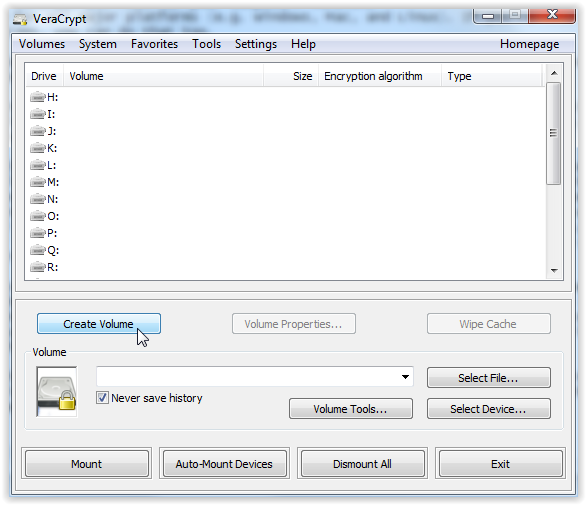
\includegraphics{imgs/VC01.PNG}

Then choose to "Create an encrypted file container."

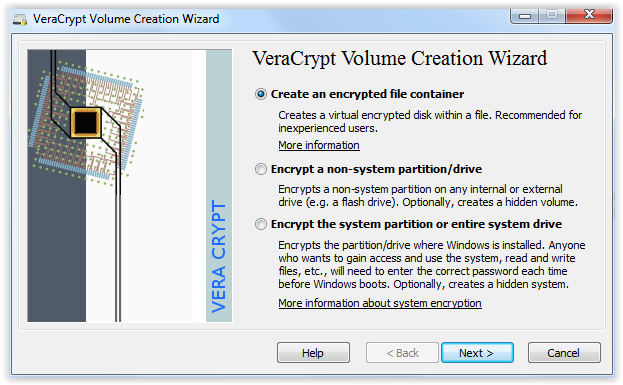
\includegraphics{imgs/VC02.PNG}

Click "Next >" until you're asked to provide the volume location. I strongly recommend not to
save history as saving the history could provide anyone with access to your computer access
to the files you've encrypted. Click "Select File..." and navigate to your main project folder.

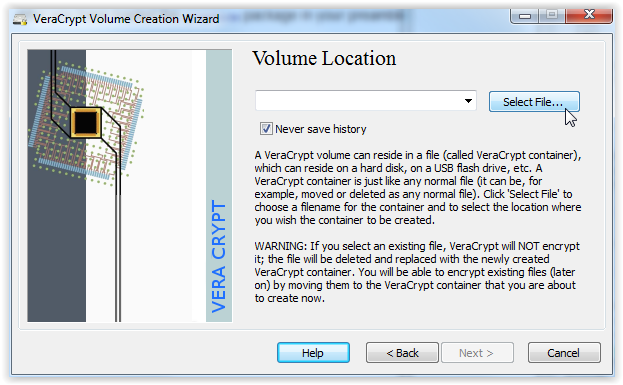
\includegraphics{imgs/VC03.PNG}

Once you're in the folder type a name for the private file (e.g. "Emotional Stroop Private")
and click "Save"

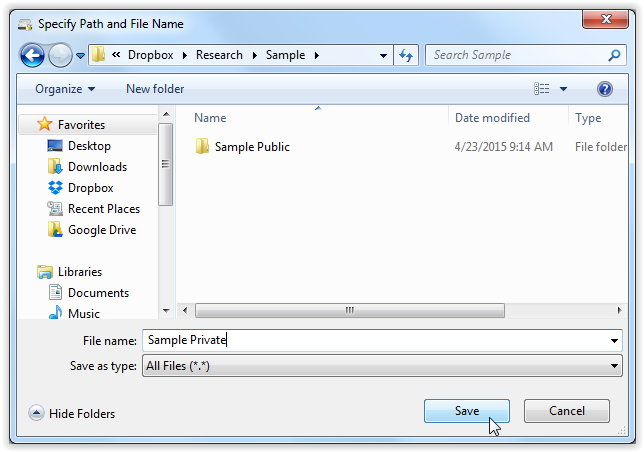
\includegraphics{imgs/VC04.PNG}

Click next until it asks you about the volume size. You'll need to select a size for the
encrypted file that should be large enough to contain all of the confidential information.
If you'll just be encrypting copies of emails, this doesn't need to be very large at all.
Go with 10 MB. If this turns out to be insufficient when you're collecting data, you can
use these instructions to create a second private folder or a larger one to contain all
the data.

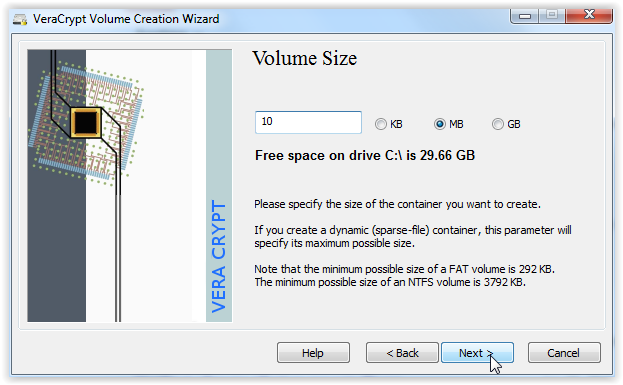
\includegraphics{imgs/VC05.PNG}

Next you'll create a password that you'll need to decrypt the file to access the confidential
information. Don't use a password you use for other files or services as this increases the
possibility that others could gain access to the confidential information. I recommend using
a \href{http://www.howtogeek.com/howto/windows/using-password-phrases-for-better-security/}
{password phrase} or a long password containing letters, digits, and special symbols for the
best security. As our memories aren't perfect, it might be a good idea to look into a
\href{http://lifehacker.com/5042616/five-best-password-managers}{password manager} such as
\href{http://keepass.info/}{KeePass}.

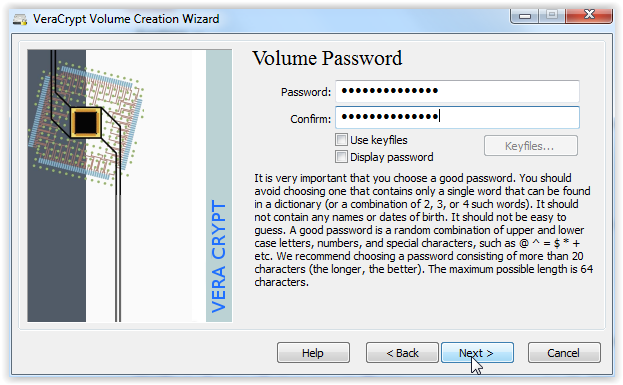
\includegraphics{imgs/VC06.PNG}

On the next screen, you'll need to move your mouse around. These movements help increase the
security of the encryption. I'd recommend moving your mouse around for about a minute. This
gets boring, so draw imaginary pictures or write invisible cursive sentences with your mouse
to help the time pass. Then click "Format".

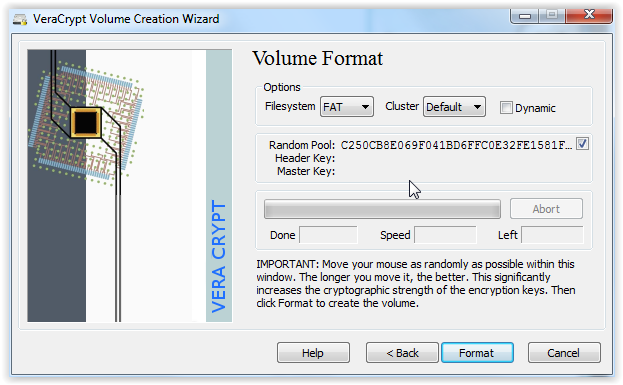
\includegraphics{imgs/VC07.PNG}

Depending on the size of the encrypted file, you may have to wait a while for VeraCrypt to
do it's thing. Once it's done creating the encrypted file. It will tell you that a Volume has
been created. Click "Next" and then close the window.

Now you have a safe repository for any confidential information.

To view, add, or remove information to this file, you'll need to decrypt it using VeraCrypt.
If VeraCrypt isn't already open, reopen it and click "Select File..."

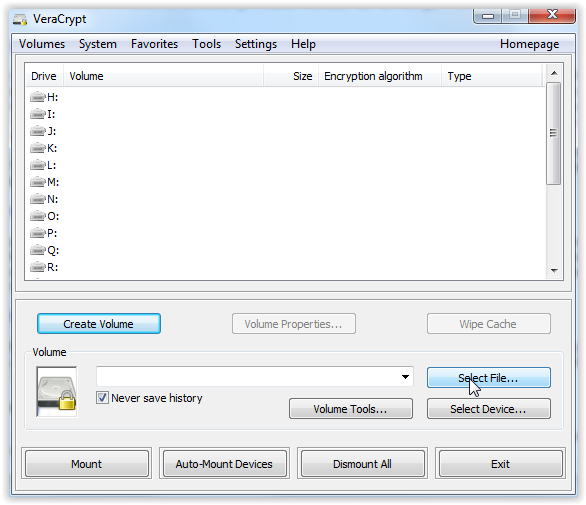
\includegraphics{imgs/VC08.PNG}

Then find the file you created, select it, and click "Open." Back in the main screen, click one
of the available drive names and then click "Mount."

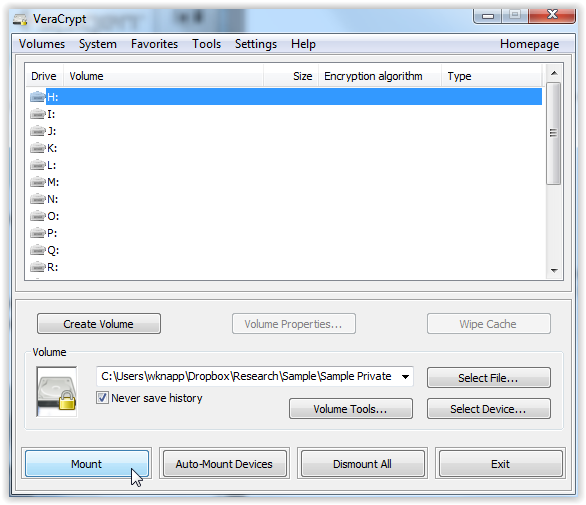
\includegraphics{imgs/VC09.PNG}

Next, enter your password and click "Ok."

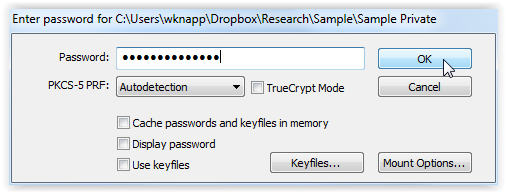
\includegraphics{imgs/VC10.PNG}

If you see the following pop up, don't be alarmed. Good encryption takes time to decrypt.

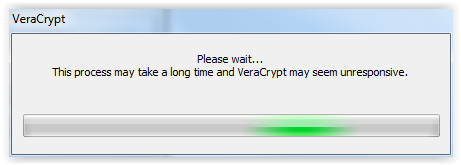
\includegraphics{imgs/VC11.PNG}

If everything went well, your file will be mounted as a virtual hard drive with the letter
you selected.

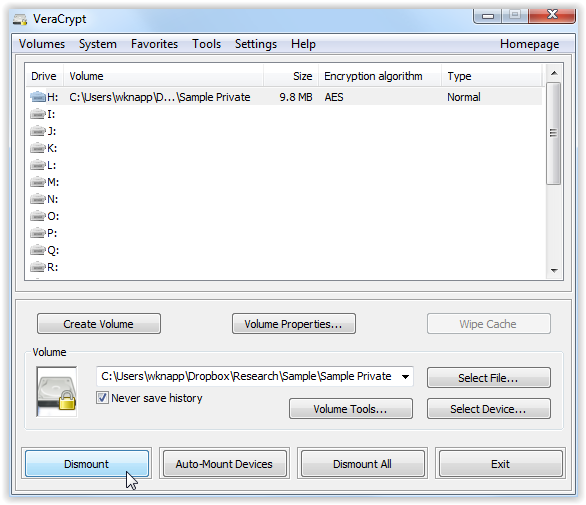
\includegraphics{imgs/VC12.PNG}

Once the file has been mounted, you can use it like any other hard or thumbdrive.

Now that you have your file mounted. You can start saving your confidential documents to
the encrypted file. If you have paper documents, I recommend scanning them and converting
them to pdf. If you have pictures or videos, you can save them directly (although you'll
need a much larger encrypted file). If you have emails, load them and print / save them as
a pdf in the mounted file.

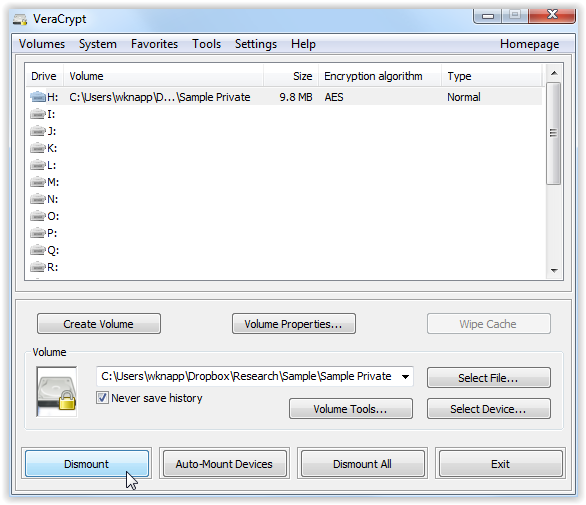
\includegraphics{imgs/VC12.PNG}

If you don't have the ability to print or save them as a pdf. Check out some
\href{http://www.cutepdf.com/products/cutepdf/writer.asp}{free software} that will allow
you to print emails and other documents as pdfs.

When you're finished saving the emails as pdfs or some other format you can access later,
make sure you dismount the encrypted file. Dismounting prevents others from accessing the
protected contents when you're away from your computer.

\subsubsection{Keeping Track of Changes Using Git}
As you collect more data, the csv file (or other files) you'll enter the data into will
grow. As you begin running analyses, the number of analyses you'll perform will also grow.
Keeping track of the changes to your data files and analyses can help you to recreate
the data or analyses at different points. This can be quite useful if you remember performing
some analysis that suggested something about the data, but you can't currently remember how
you did it.

To keep track of changes to our data, analyses, and / or other files, we're going to use a
\href{http://en.wikipedia.org/wiki/Revision_control}{version control system}. You all had
experience with a version control system when you were working with
\href{https://docs.google.com}{Google Docs} (Gdocs) last semester. Gdocs tracked every change
or suggestion that you, I, or your peers made. We're going to do something similar, except
we're going to track changes for an entire folder of information.

To accomplish this, you'll need to download and install the version of
\href{http://git-scm.com/downloads}{Git} that will run on
your computer. Like VeraCrypt, Git is open source and free. It has a huge user community.
Although it started as a way to track changes in code used to create software, it's been
adopted to track changes in a variety of applications, including psychological research. It
has a huge user community, so it's pretty easy to find help online if you're having trouble
with something. Again, use the defaults unless you know what you're doing.

Unlike most programs you're probably familiar with, Git is a
\href{http://en.wikipedia.org/wiki/Command-line_interface}
{command line program} in which you'll need to enter commands. If you haven't used such
a program before, don't worry. We'll cover all the commands you need to use to accomplish
what you need for this class. It's really no harder than pointing and clicking once you
know what you're doing.

Git should install itself with two options to run it. Git GUI and Git Bash. We'll be using
Git Bash for this assignment. The following image comes from my list of programs on a
Windows PC.

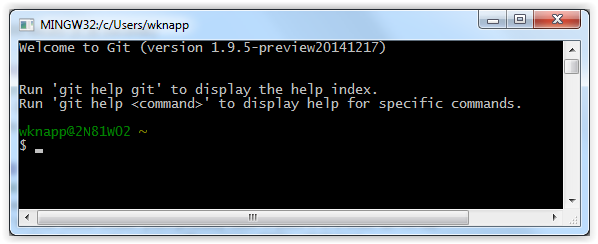
\includegraphics{imgs/Git01.PNG}

When you first fire up Git Bash, you should see a window that looks like this:

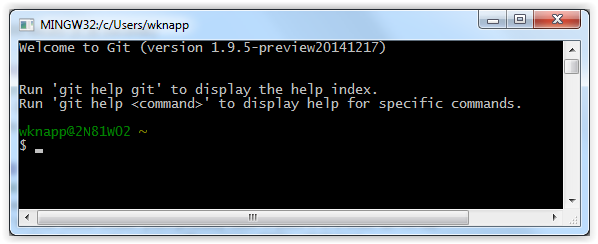
\includegraphics{imgs/Git02.PNG}

Notice the title ``MINGW32:/c/Users/wknapp'' at the top the window. You'll see something
different based on your home directory on your computer. ``MING32:''
isn't important for us, but the ``c/Users/wknapp'' is as it indicates what
directory you're in. As you navigate around in Git, this title will change so you'll
always know where you are. This is good because the first thing we need to do is
navigate to the public folder. To move around, we'll be making heavy use of the cd
(i.e. change directory) command. Let's get a little practice moving around.

To help you, I'll type in examples of commands using names for my files and folders.
You should follow along with me and replace my file / folder names with yours. Code
that you should enter will be formatted as follows:

\begin{verbatim}
$ ls
\end{verbatim}

The dollar sign indicates that Git is waiting for you to enter commands. Thus, the 
first command I issued was ``ls'' (list files). When you see code blocks, like
above, just type in what follows the dollar sign. As you can see, one of the files is
``Dropbox,'' which is actually a folder that contains my sample project.

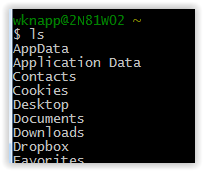
\includegraphics{imgs/Git03.PNG}

I want to change directories to be inside the Dropbox directory. \textbf{TIP:} You'll have
different files and folders on your computer, so you'll need to adjust the commands to
navigate your file structure. Otherwise, you'll be trying to navigate mine, which is
highly unlikely to work.

\begin{verbatim}
$ cd Dropbox
$ ls
\end{verbatim}

The dollar sign indicates that Git is waiting for you to enter commands. Thus, the 
first command I issued was ``ls'' (list files). As you can see, one of the files is
``Dropbox,'' which is actually a folder that contains my sample project.

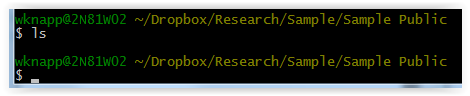
\includegraphics{imgs/Git04.PNG}

Notice how after I changed the directory, the line above the \$ prompt changed from
ending in a tilda (i.e. ``~'') to ending in a tilda followed by a forward slash (i.e.
``/'') and the name of the directory I changed to. The tilda represents my home
directory (i.e. c:/Users/wknapp). The forward slash represents a subdirectory, with
the name of the subdirectory following the slash.

After navigating to the Dropbox directory, I again used ``ls'' to see what was there.
You can see there are files (e.g. Abuse.docx) and folders (e.g. 111AAA). From the Dropbox
folder, I want to go three folders deeper into my ``Sample Public'' folder. I can change
into any deeper directory by separating the different names of the directories with
forward slashes.

\begin{verbatim}
$cd "Research/Sample/Sample Public"
\end{verbatim}

Notice that I used quotes around the list of subdirectories that I wanted to navigate.
The reason I did this is because the final directory had a space in the name (i.e.
Sample<space>Public). Without using the quotes, Git would have thought that I was
issuing another command after Sample.

Let's start back in our home directory so we can see three ways of navigating to the same
place. To get back to the home directory use the following command:

\begin{verbatim}
$ cd ~
\end{verbatim}

Remember that ``~'' represents the home directory, so we can use that directly. Now that
we're back home, lets see three ways of doing the same thing. You can use the way that
makes the most sense to you.

\begin{verbatim}
$ cd Dropbox
$ cd Research
$ cd Sample
$ cd "Sample Public"

     or
     
$ cd "Dropbox/Research/Sample/Sample Public"

     or

$ cd "c:/Users/wknapp/Dropbox/Research/Sample/Sample Public"
\end{verbatim}

The last example is useful if you already know where something is and it's not
located somewhere inside your home folder.

So navigate back to your project directory and list the files.

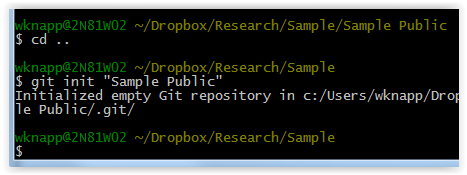
\includegraphics{imgs/Git05.PNG}

The list should come up empty and return you to the prompt since there aren't any files
in your project directory yet. We can create files and folders directly in Git, but
since you're all probably more familiar with using the file manager already on your
computer, feel free to use that.

We want to tell git to use our public project directory, but we need to do this in the
directory above the project directory. Thus we need to move up one level in the
directory structure. This is surprisingly easy to do.

\begin{verbatim}
$ cd ..
\end{verbatim}

The two periods tell Git to go up one directory level. Now that we're in the main project
directory, we can tell Git we want it to track changes in the public project directory
using the initialize command init

\begin{verbatim}
$ git init "Sample Public"
\end{verbatim}

Git will quickly do its thing and return you to the command prompt.

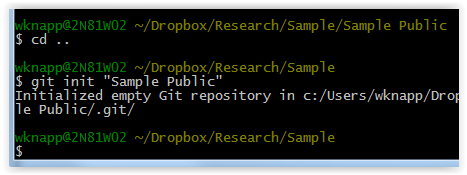
\includegraphics{imgs/Git06.PNG}

Now all that's left to do is to create any directories you need. I'd recommend using the following
structure for directories and files for your capstone project. Of course, you can use different,
hopefully more descriptive, names. You're also free to use a different structure that makes more
sense to you. What's important is that it's easy to find what you're looking for and that
everything is in place to allow others to reproduce your results with your data or replicate
your experiment with your materials.

\begin{itemize}
\item materials (directory)
    \begin{itemize}
    \item IRB Application (file)
    \item IRB Approval Letter (file)
    \item Informed Consent (file)
    \item Debriefing (file)
    \item Any materials you used (files: e.g. surveys). If you conducted a YouTube experiment,
        I'd recommend creating a file that provides links for the consent, debriefing, and all
        conditions.
    \end{itemize}
\item data (directory)
    \begin{itemize}
    \item data.csv (file containing non-confidential data you'll analyze)
    \item codebook.md (file providing descriptive codes for the data in your data.csv file)
    \item analysis.Rmd (file containing analyses, descriptions of analyses, and code you used
        to create any figures or tables)
    \item figures, graphs, and tables (files that will be produced automatically when you process
        your analysis.Rmd file)
    \end{itemize}
\item presentation (directory)
    \begin{itemize}
    \item presentation.pptx (presentation file---can be in
        different formats based on what you have available)
    \item presentation.pdf (a pdf version of your presentation suitable for printing at
        poster size)
    \item watchpresentation.txt (a file containing a link to your video walk through of the
        presentation)
    \end{itemize}
\item README.md (file that briefly overviews the project and explains what the directories are
    and what they contain)
\end{itemize}

There are probably some file extensions you haven't seen before (e.g. Rmd and md), but we'll get
to those shortly.

I've added a couple directories and a README.md file to my Sample Public folder for Git to track.

Now that I've reached a good stopping point, I'll tell Git to pay attention to what I have now.
Although Git tracks changes, it only tracks changes when you tell it you have changes you're committed
to. This means that it won't track each time you enter a symbol or use backspace. This is great news
if you type like I do and regularly have to backspace and make corrections.

To tell Git to add all that we've done to it's list of things to track use the following command.

\begin{verbatim}
$ git add -A
\end{verbatim}

The ``-a'' tells git that we want to add everything we've created in the tracked directory and
the subdirectories. You don't have to add everything, but I'm trying to keep things simple for this
project.

Although git now knows that you want to track everything in the public directory. It won't actually
track any changes until you tell it that you're committed to the current version of the files you have.
To do this, use the following command from inside the directory you initialized.

\begin{verbatim}
$ git commit -m "Initial commit of my sample project"
\end{verbatim}

All we really have to do to let Git know that we're committed to what we have is to say \emph{git commit}.
But as your project goes and you make multiple commits, you might want to take a look at a particular
commitment. Thus we use ``-m'' to add a message to our commit, which we provide in quotes. These
messages should be descriptive (e.g. ``added initial analyses'', ``ran additional t-tests'', or 
``completed presentation''). Then you or others can quickly see how your project has evolved over time.
If you're really interested in maximizing the potential of commit messages, which is well beyond the
scope of this course, check out
\href{https://robots.thoughtbot.com/5-useful-tips-for-a-better-commit-message}
{5 useful tips for a better commit message}.

Each time you've finished a piece of your project, I'd recommend using both commands.

\begin{verbatim}
$ git add -A
$ git commit -m "Descriptive message here."
\end{verbatim}

\subsubsection{Freeing the Data with Github}
To make a project fully reproducible and replicable, you need to give others access to your materials,
data, and analyses. To do this, we're going to use a free online service that integrates nicely with
Git: \href{https://github.com/}{Github}.

Now Github presents an interesting challenge for Educators who are bound by
\href{http://www2.ed.gov/policy/gen/guid/fpco/ferpa/index.html}{FERPA} to protect the identities
of their students and not release any identifiable student work without the student's permission.
Thus, if I'm going to ask you to make your work visible to the public, it needs to be possible
to do so in a way that protects your identities.

To successfully complete the project, you'll need to sign up for a Github account. However, when
you sign up, you do not have to use your name anywhere on your account. You can sign up with
whatever username you like (e.g. william\_knapp or CheesyPoofMaster83). You can also sign up with a
\href{http://www.throwawaymail.com/}{throwaway email address}. You are entirely free to use your
name and email. In fact, I'd encourage you to do so in certain situations. However, your grade
will not depend on your choice to hide or reveal your identity. Furthermore, as you have control
over whether or not you reveal your identity, such a revelation will be considered as permission
to make your work visible. I won't post grades on the site, so you needn't be concerned that
your confidential grades will be released.

If you're taking the project seriously and are proud of your work, revealing your identity offers
potential employers or admissions committees tangible evidence of the skills you
claim to have in application documents. They'll be able to see first hand that you know how to
design an experiment, use R, perform analyses, and create graphs and presentations.

If you're just doing what you need to do to pass, revealing your identity could be embarrassing
and actually hurt your chances at securing employment or getting into graduate programs.
I would not suggest using identifiable information unless you're proud of what you're doing.

Although you need to sign up and use Github for this course, you are free to
\href{https://help.github.com/articles/deleting-your-user-account/}{delete your account} or
\href{https://help.github.com/articles/deleting-a-repository/}{delete your project} at the end
of the semester regardless of your decision to reveal or hide your identity.

As some of the materials include personally identifiable information (e.g. a YouTube video with
your email address or a debriefing form), if you or your partner do not wish to reveal your
identities, you're free to complete the project without providing those materials. Instead, you
could create a description of what would have been there otherwise (e.g. ``A link to the
$\rule{1cm}{0.15mm}$ condition [link removed to protect the authors' identities]'' or 
``Authors' information redacted'').

To sync what you've committed with Git to Github, first you'll need to create an online repository
(i.e. project). So sign up for Github after strongly considering whether you want to reveal
or conceal your identity. Then log in. At the upper right corner of the screen, you'll see your
user name and plus sign with a downward facing triangle. Click that and then click ``New
repository''.

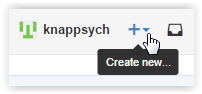
\includegraphics{imgs/Github01.PNG}

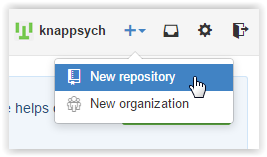
\includegraphics{imgs/Github02.PNG}

Then you can enter a name and description for your project. Using the same name as your public folder
is a good idea, so I went with that. You'll notice that when I entered ``sample public'' it was changed
to ``sample-public.'' This change was made so you have a \href{http://www.desiquintans.com/cleanurls}
{pretty URL} to your project. Browsers transform spaces into a special code that would make your URL
less pretty (i.e. ``sample\%20project''). Don't initialize the project with a README as you'll be making
your own. Unless you pay Github, you'll have to make the project public. For this class don't worry
about .gitignore or licensing. When you're finished, click ``Create Repository.''

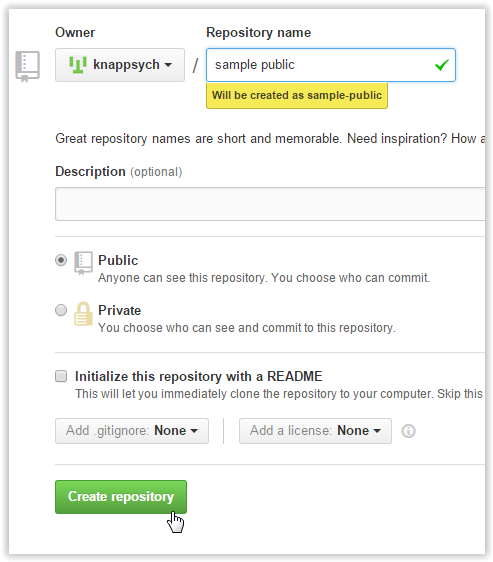
\includegraphics{imgs/Github03.PNG}

Now that you have a project on Github, you can sync the files on your computer with Github. This is
awesome because it means that if your hard drive crashes, the data are still out there in the cloud.

Syncing your local folder with Github is pretty easy. In fact, after you've created your project on
Github it will provide you with the commands you'll need to accomplish this once you're inside the
local folder that Git is tracking.

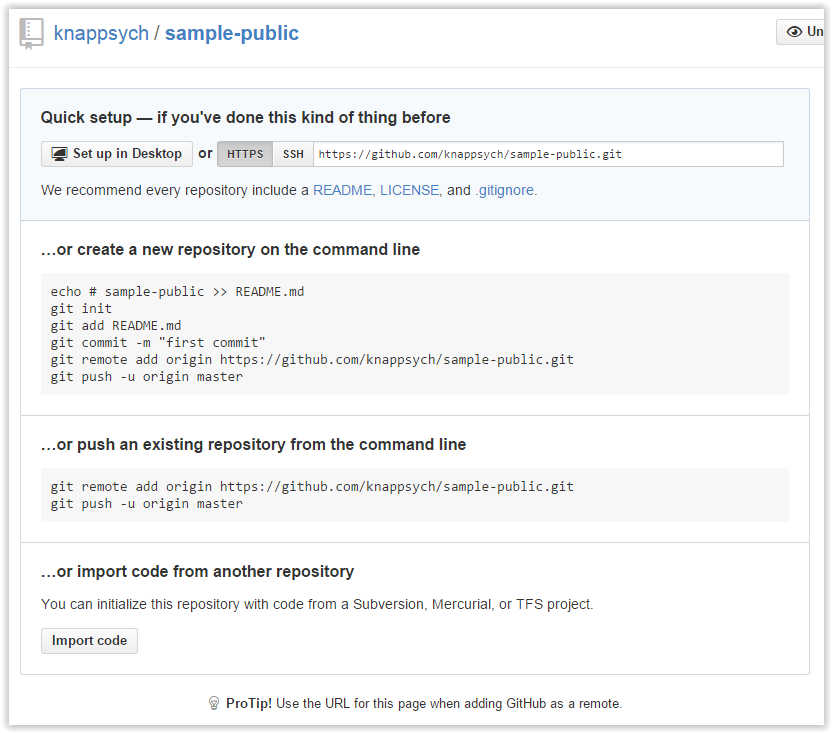
\includegraphics{imgs/Github04.PNG}

To sync your local folder with Github, go to the directory Git is tracking. Then type in the
following code. Note that pasting doesn't necessarily work in Git, so you might have to type
everything. Also note that I've broken up a single command onto two lines so you can see
everything. In Git, the URL should come after origin (e.g. ``...origin https...'').

\begin{verbatim}
$ git remote add origin
      https://github.com/yourusername/yourprojectname.git
$ git push -u origin master
\end{verbatim}

At this point, Git will prompt you for your username and password. If you've done everything properly,
Git will do it's thing and give you information about what files it uploaded and how many lines
it changed.

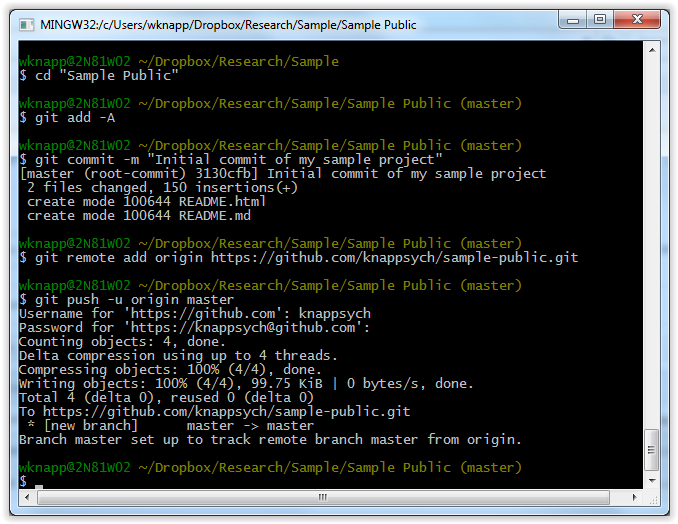
\includegraphics{imgs/Github05.PNG}

Once Git is done, go online and see whether your project is there. If you've done this after creating
the README.md file (see next section), you should see something like this.

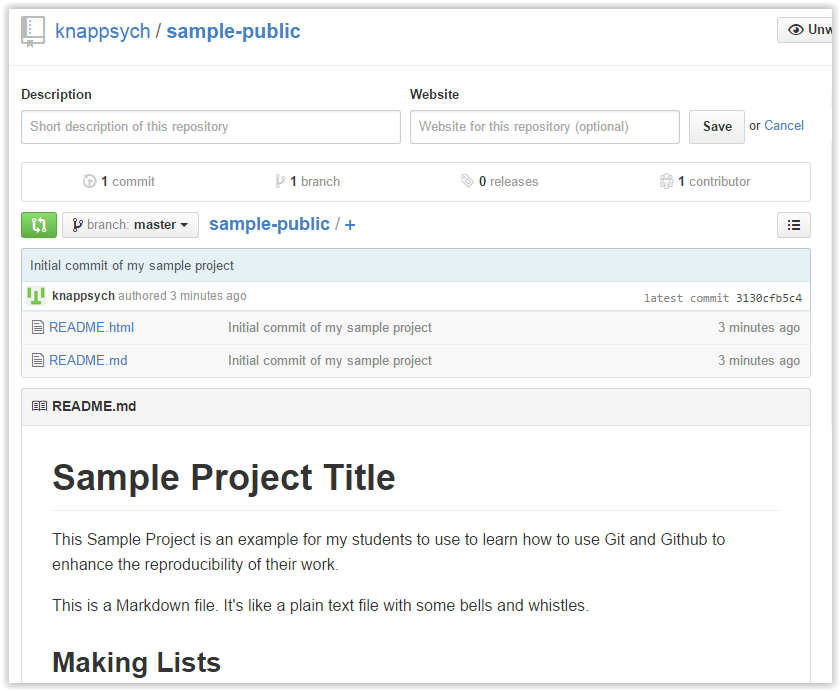
\includegraphics{imgs/Github06.PNG}

\subsubsection{Standing on the Backs of Giants}
I'm certainly not a giant, but opening our data allows others to benefit from our work in addition to
checking whether our analyses are reproducible or our studies are replicable. In addition to making
your work available to others, Github allows you to build your own projects based on the work of
others. If you see something you like on Github, feel free to take it and modify it. You should
give credit to those whose work you use, but if you take it by creating a Github fork, Github will
identify the project that your work comes from.

Think of Github forks as forks in a road. Someone has a project, but you want to take it in a new
direction. Rather than reinventing the real, you can ``fork'' their project which recreates the
project for your account. Then any changes you make to the project can be easily tracked. If
you make some awesome changes for a computer program, you could work with the original project owner
to integrate your work.

For your homework assignment, you'll need to fork
\href{https://github.com/knappsych/capstone-reproducibility}{my project for this class}. Forking is
incredibly easy. Just go to the website once you're logged in. Then look for the symbol that looks
like a fork in a road in the upper right hand corner of the page.

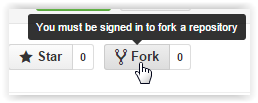
\includegraphics{imgs/Github07.PNG}

If you're logged in, you won't the message to log in and you'll instead be prompted to ``Fork your
own copy of knappsych/capstone-reproducibility to your account.'' Click it and Github will take you
to your newly forked project.

When you go to your newly created project you'll see that that there is a data directory and a
README.md file. The README.md file will briefly explain what's in the other
directory. So you don't have to check the README now, the data directory contains the following:

\begin{changemargin}{3.2cm}{0cm}
\begin{itemize}
\item [politics.csv] The file you'll need to complete the homework
assignment.
\item [Generation.Rmd] The file I used to create the data file.
The data were generated in a fully reproducible way, so if you process Generation.Rmd on your own
computer, you should be able to regenerate the file for yourself.
\item [Example.Rmd] A model for the homework assignment you'll
need to complete. In it, I'll perform a number of the analyses and create the figures that you'll see
later in this text. The primary difference between what you'll see in this text and what you'll see
in the Example.Rmd file is that I walk you through things here, but I won't there.
\item [Homework.Rmd] The file you'll need to fill in to successfully complete the assignment before
syncing it to your \href{https://github.com/knappsych/capstone-reproducibility}{fork of my project}.
Homework.Rmd is bare bones, so I strongly recommend referring to Example.Rmd as you work through the
problems.
\item [Codebook.Rmd] A file that explains what the variables
in the data set are. You don't need to do anything to this file for this assignment, but it will be
useful to use it as a template for the data for your own study in completing your capstone project.
\item [Reproducibility.pdf] This document!
\item [Reproducibility.Rnw] The file that was used to create this document
inside RStudio. If you want to try for yourself, go for it, but you'll have to install \LaTeX on your
computer.
\item [imgs] A directory including all the images for this text.
\end{itemize}
\end{changemargin}

Together, these files make the assignment completely open and reproducible. Yeehaw!

Once you've forked the project, you'll need to download the information to your computer so you can alter
it and push your changes. To accomplish this you'll need to create a folder for the reproducibility
and statistics assignment. I called mine ``reproducibility.'' After cd'ing to your assignment folder
and initializing it, all you need to do is ``pull'' down the data. When you have something you want
to upload, you push. When you want to download you pull. There are some other 
\href{http://longair.net/blog/2009/04/16/git-fetch-and-merge/}{options too}, but I'd
stay away from them for this project unless you want to become a Git Guru---I'm just a Git Guppie.
\textbf{TIP:} you need to be in your initialized assignment directory for the following to work the
way you probably want it too. If you do this in your project directory, you'll fill up your project
with a bunch of unrelated files.

\begin{verbatim}
$ git pull https://github.com/your-user-name/capstone-reproducibility
\end{verbatim}

If everything works, you should see something like the following.

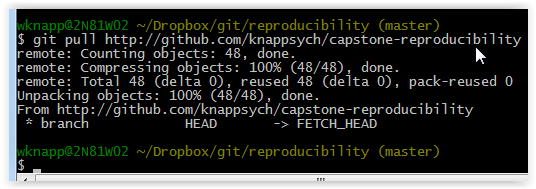
\includegraphics{imgs/Github08.PNG}

\subsubsection{Explaining the Data with Markdown}
\href{http://en.wikipedia.org/wiki/Markdown}{Markdown} is an incredibly easy language to use for
documenting your work. You write Markdown in plain text and use a few special symbols or conventions
to create organization to your document. Although there are lots of bells and whistles, we're only
going to need a few to make your assignments easy to read. Specifically, we'll take a look at titles,
bold, italics, links, and lists.

Creating a Markdown file is easy. Just open up a plain text editor (we'll use the one contained in
RStudio) save the file with a .md extension and start typing. The .md extension tells Github and
other programs that it's a plain text file that follows some conventions. Github and other programs
take the .md file to create a simple webpage that's formatted according to the conventions. 

Let's take a look at the conventions you're most likely to need to use for your Capstone project. To
create titles and subtitles, just start the line you wish to emphasize with one or more pound signs
(i.e. ``\#'').

\begin{verbatim}
#Title
##Subtitle
###Subsubtitle
\end{verbatim}

To create an unordered list, start each list item with an asterisk and space.

\begin{verbatim}
* Some item.
* Another item.
* Different item.
\end{verbatim}

To create an ordered list, start each list item with a number, period, and space.

\begin{verbatim}
1. First.
2. Second.
3. Third.
\end{verbatim}

To add special formatting like links, italics, or bold. Use the following conventions.

\begin{verbatim}
Here's a [link](https://www.google.com/).
*italics*
**bold**
***bold italics***
\end{verbatim}

The one other thing you should know is that that when you end a paragraph by pressing
enter, Markdown will treat that as a space. This
is a good thing. In many text editors, if you don't press enter, your line will
continue to the right. This would make reading or editing a plain text file a pain as
one would regularly need to scroll to the right or the left. So to create a paragraph
that doesn't extend beyond the margins of your window, just press enter after you've
typed around 80 characters.

To create new paragraphs, simply press enter twice. You don't need to do this for lists,
but you will otherwise. Let's see how all of this works in an example.

\begin{verbatim}
#Markdown Example

##Creating Lists

###Unordered Lists

* One thing in *italics*.
* Something else in *bold*.
* A [link](http://phdcomics.com) to a great webcomic.

###Ordered Lists

1. First
2. Second

##Paragraphs

This is all
a single paragraph.

Notice the blank line separating paragraphs.
\end{verbatim}

After being processed, the result should look something like the following.

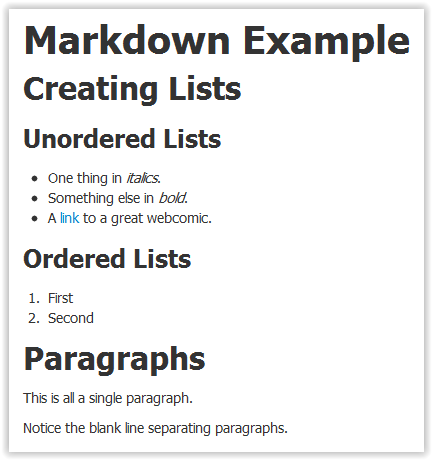
\includegraphics{imgs/md01.PNG}

\begin{comment}
\begin{changemargin}{0cm}{0cm}

\begin{mdh1}Markdown Example\end{mdh1}

\begin{mdh2}Creating Lists\end{mdh2}

\begin{mdh3}Unordered Lists\end{mdh3}

\begin{mdstyle}
\begin{itemize}[leftmargin=.7cm,itemsep=0pt,parsep=0pt]
\item One thing in \emph{italics}.
\item Something else in \textbf{bold}.
\item A \href{http://phdcomics.com/comics.php}{link} to a great webcomic.
\end{itemize}
\end{mdstyle}

\begin{mdh3}Ordered Lists\end{mdh3}

\begin{mdstyle}
\begin{enumerate}[leftmargin=.7cm,itemsep=0pt,parsep=0pt]
\item First.
\item Second.
\end{enumerate}
\end{mdstyle}

\begin{mdh3}Paragraphs\end{mdh3}

This is all a single paragraph.

Notice the blank line separating paragraphs.
\end{changemargin}
\end{comment}

\subsubsection{Analyzing the Data with R Markdown}
\href{http://rmarkdown.rstudio.com/}{R Markdown} is basically just Markdown with the
ability to process R code. Just as there are simple conventions to create titles,
lists, and formatted text, there are simple conventions to mark R code for processing.
To create an R Markdown file, we do the same things we did to create a markdown file,
except we give it a file extension of .Rmd instead of .md. Simple as pie!

Let's first take a look at how to show your R code and / or the resulting output in
separate blocks.

\begin{verbatim}
```{r}
# This is an R comment that R will ignore.
# Because these comments are in an R block, they won't be
  # confused with Markdown titles.
# R code goes in here.
# The ```{r} on its own line starts the R code section.
# The ``` on its own line ends the R code section.
```
\end{verbatim}

If you tried to run the above without making them comments, you'd get some errors because
I didn't use used proper R code inside the block. But, hopefully, you have the idea.

Had there been uncommented real code, the previous would
have resulted in blocks of R code and the results of the operations performed in
the code. This is fine for some purposes, but there are times that you might only
want the results (e.g. when you're creating a figure) or only want the code (e.g. when
the results go on and on). Other times, you might want to store the results of some
operations (e.g. you're running massive simulations that take hours) so you don't 
have to perform the operations each time. Fortunately, R Markdown makes all of these
possibilities a breeze.

All you need to do is change the first line of the R code block. See the following
examples:

\begin{changemargin}{5cm}{0cm}
    \begin{itemize}
    \item [Output Only:] \begin{verbatim}```{r, echo=FALSE}\end{verbatim}
    \item [Code Only:] \begin{verbatim}```{r, output="hide"}\end{verbatim}
    \item [Both:] \begin{verbatim}```{r}\end{verbatim}
    \item [Neither:] \begin{verbatim}```{r, include=FALSE}\end{verbatim}
    \item [Store Results:] \begin{verbatim}```{r, cache=TRUE}\end{verbatim}
    \end{itemize}
\end{changemargin}

It's important to note that if you're creating a figure, hiding the output won't
hide the figure. However, not including the block by setting include to FALSE will.

Sometimes, you might want to include the result of an R calculation directly into the
text. This is also easy to accomplish. All you need to do is surround the R code with
back quote symbols and indicate you're using R code by starting the code with ``r''
and a space. For example:

\begin{verbatim}
The mean of 1 and 2 is `r mean(c(1,2))'.
\end{verbatim}

Don't worry about the specifics of the R code yet. We'll get there shortly. But let's
take a look at what an R Markdown file looks like when you type it and after it's
processed.

\begin{verbatim}
#R Markdown Example

####Code and Output
```{r}
#Let's create a sample n-10 from a normal distribution
      #mean 5 and standard deviation 2
sample<-rnorm(10,5,2) #Assigns the sample to 'sample'
sample #Shows us what's in the sample
```

####Output Only
```{r, echo=FALSE}
a<-mean(sample) #assigns the mean of our sample to a
a #shows us what's in a
```

####Code Only
```{r, results="hide"}
a
# Hiding results won't hide figures
```

####Neither Code Nor Output
```{r, include=FALSE}
a
# Using include=False will hide figures
```
Notice how there's no block for code or output.

####Caching Information with Code Only
```{r, cache=TRUE, results="hide"}
b<-a+2 #Adds 2 to a and assigns that value to b
a
```

####R Results in Text
The mean of x is `r a`.
The mean of x is `r mean(sample)`.
The mean of x is `r b-2`.
The mean of x is `r sum(sample)/length(sample)`.
\end{verbatim}

After the file is processed, it will look something like this.

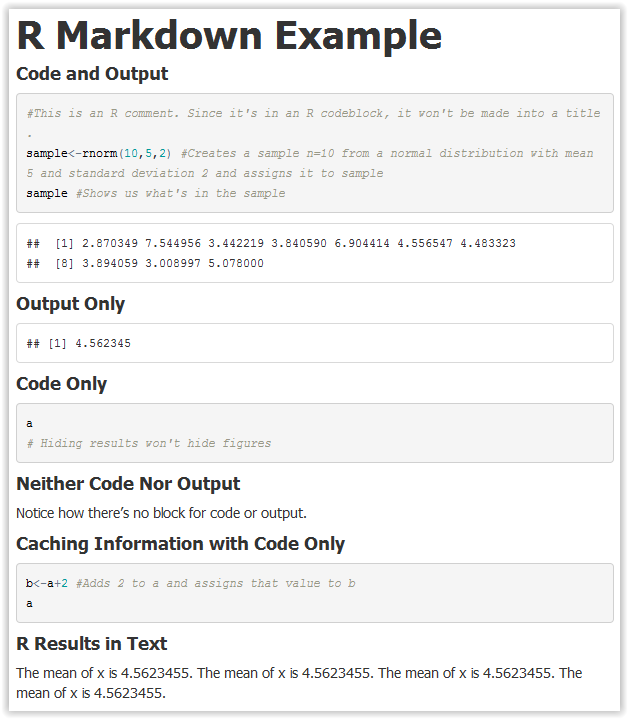
\includegraphics{imgs/Rmd01.PNG}

\section{Using R in RStudio}
\href{http://www.r-project.org/}{R} is an incredibly powerful tool in any data
scientist's toolbox. R can be used to analyze data, run simulations, create
figures, and even create documents. Except for the screenshots, this entire
document was created using R in RStudio.

\href{http://www.rstudio.com/}{RStudio} is an
\href{http://en.wikipedia.org/wiki/Integrated_development_environment}
{integrated development environment} that simplifies working in R. Together
R and RStudio are a powerful combination that can be used in any of the ways I've
mentioned in a way that can dramatically enhance reproducibility. We can use this
combination to create our .csv, .md, and Rmd files we'll use to hold our data,
explain our project, and analyze our data.

\subsection{Installing R and RStudio}
To download R, pick a mirror (i.e. a location that holds the files you want) from
\href{http://cran.r-project.org/mirrors.html}{this list} that's close to your
location. Once you've picked a mirror, choose the version of R that's appropriate
for your system (e.g. Windows, Mac, or Linux). Download the installation file and
install R. I recommend using the defaults unless you know what you're doing.

Once R is installed, \href{http://www.rstudio.com/products/rstudio/download/}
{download} the version of RStudio you need for your computer. Again, use the
defaults unless you know what you're doing.

\subsection{Working in RStudio}
Once you're finished installing both programs, fire up RStudio for the first time. You should see something like the following.

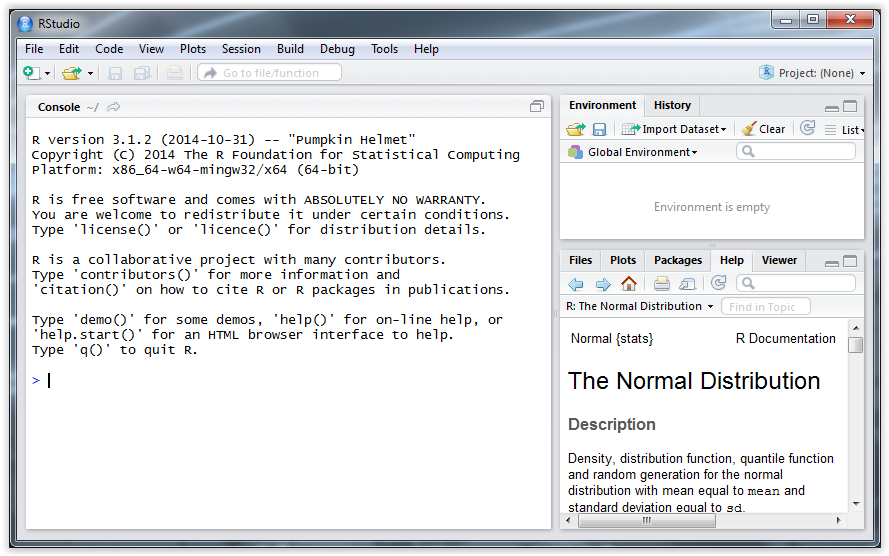
\includegraphics{imgs/R01.PNG}

Before we take a look at the different sections inside RStudio, I'd like you
to create an R Markdown file. This is incredibly easy to accomplish. Just
click on the far left icon under the tool bar that looks like a blank page
with a plus sign in a green circle. Then click ``R Markdown...''

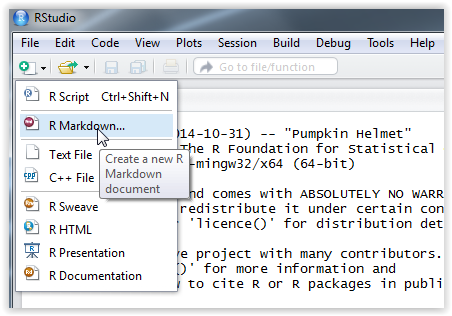
\includegraphics{imgs/R02.PNG}

This will open up a dialog where you can add a title and your name to the
document. Go ahead and enter whatever you'd like. Remember, for the homework
and capstone project, you'll be posting these files on Github. So don't use
your name if you want to conceal your identity.

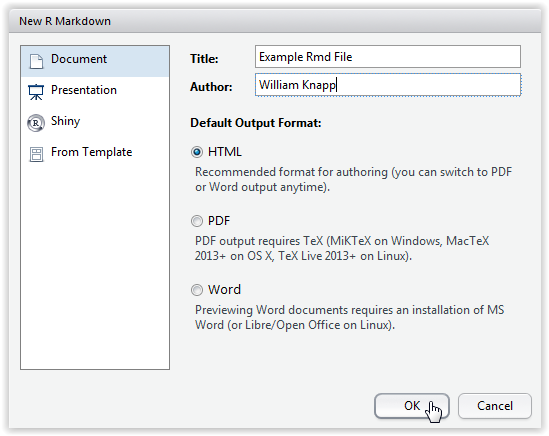
\includegraphics{imgs/R03.PNG}

After you click ``Ok,'' RStudio will automatically create an Rmd file with
a template that shows you how to include R code. Sweet, huh? Dude!

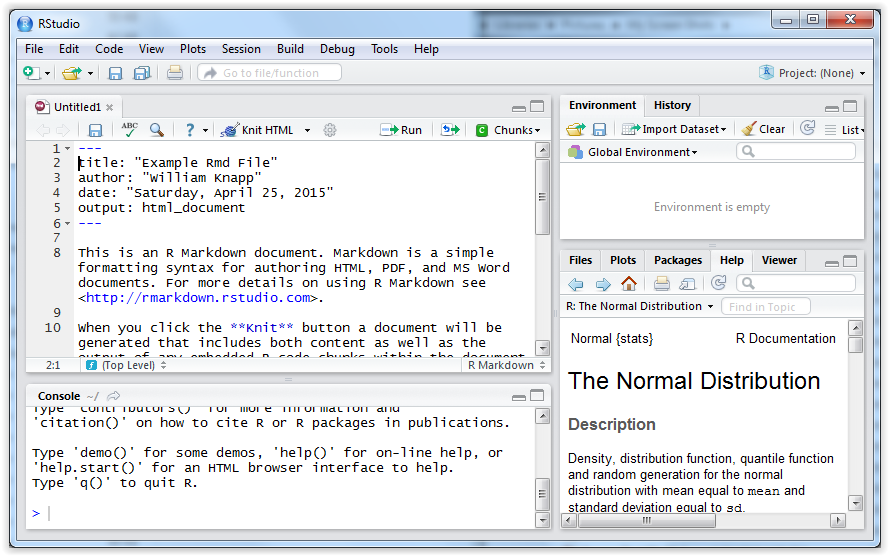
\includegraphics{imgs/R04.PNG}

\subsubsection{RStudio Sections: Code}
The code section is in the upper left hand portion of the window. The code section
is used to write reproducible code. The code is reproducible, because we can save
the files we create in this section once we have some code we want to keep. Once
you have some code in this section, RStudio will remember what you're working on
and open it up the next time you open the Program. That said, make sure you save
your work regularly so there aren't any regrets should your computer or RStudio
crash.

I recommend saving your code in a directory that Git tracks and that you're syncing
with Github. This will ensure that a catastrophic disk failure on your computer
doesn't destroy. Make sure you \emph{add} and \emph{commit} your work to Git and then 
\emph{push} them to Github when you're happy with your progress.

\subsubsection{RStudio Sections: Environment / History}
The environment and history section is in the upper right corner. We won't use this
section much. All the commands that R processes get logged in the history. The
environment tab keeps track of the variables R currently has in memory. This can
be useful if some piece of code isn't working and you want to see if the variable
it's supposed to work on is there. You can also quickly see what types of variables
you have and how much information they contain.

\subsubsection{RStudio Sections: Help, Plots, and More}
You can find help, view figures, and more in the section in the bottom right corner.
We aren't going to work much with the Files, Packages, or Viewer tabs, but we'll
use the Help and Plots tabs when we need information about R functions or create
figures, respectively.

when you create a figure or ask for help, RStudio will automatically switch to the
right tab to make things easy for you.

\subsubsection{RStudio Sections: Console and Feedback}
The console section at the bottom left corner of RStudio is where R resides. If
you ran R outside of RStudio, the console would be all that you saw until you
asked for help or created a figure.

This is where the R commands are processed. You can run commands from the code section
by highlighting code you want to run and pressing ``Run'' or by entering code directly
into the console.

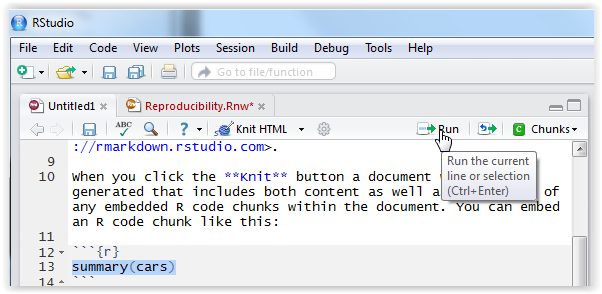
\includegraphics{imgs/R05.PNG}

\begin{verbatim}     or\end{verbatim}

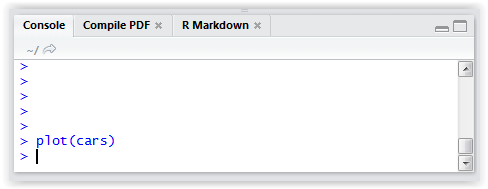
\includegraphics{imgs/R06.PNG}

If you process any type of Markdown files, this console will also show feedback about
the progress of the conversion. If you've made mistakes, they'll be noted here.

Speaking of processing a Markdown file, let's process the one that RStudio created for
us a little bit earlier. Do you see the icon that looks like a ball of yarn with some
crochet needles next to the text "Knit HTML?" Click that.

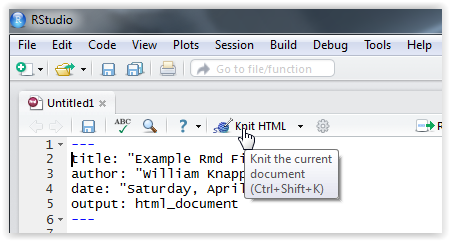
\includegraphics{imgs/R07.PNG}

If everything worked, a window should pop up that shows you what the R Markdown looks
like once it's been processed. It should look something like this:

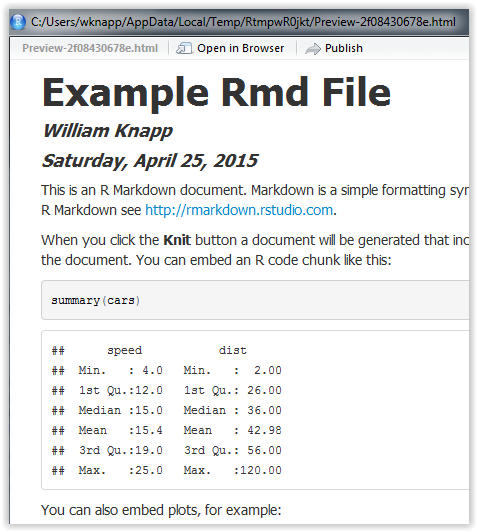
\includegraphics{imgs/R08.PNG}

You should also see a tab labeled ``R Markdown'' in the console section.

\subsection{R: Getting Help}
Starting off in R, there will undoubtedly be some things that you'd like to do but
don't yet know how. You'll probably make some errors too. In either situation
R's help and the internet can come in immensely handy. Fortunately, there are a number
of ways to find help. The box below contains raw R code based off the help from
\href{http://www.statmethods.net/interface/help.html}{Quick-R}, formatted much like what
you'd see using R Markdown.


\begin{Schunk}
\begin{Sinput}
> help.start()          #general help
> help(somefunction)    #help about somefunction
> ?somefunction         #same thing 
> apropos("test")       #list functions with test in the name
> example(somefunction) #show an example of somefunction
\end{Sinput}
\end{Schunk}

Sometimes you might not find what you're looking for. In situations like this, I
recommend turning to your favorite search engine and succinctly describing what
you want to do. Queries like the following have helped me a great deal over
the years.

\begin{itemize}
\item R create grouped bar graph ggplot2
\item R summarize data dplyr
\item R t-test tutorial
\item R regression analysis
\item R error in rbinom argument "size" is missing, with no default
\end{itemize}

One tip, the actual R documentation can be a royal pain to read if you're
not used to it, so feel free to search the internet if you're having trouble after
reading the R documentation. I have personally found answers at
\href{http://stackoverflow.com/questions/tagged/r}{stack\textbf{overflow}} or in
blog posts to be much more comprehensible than much of the R documentation.

If you can't find anything, you can ask a question. A good question will 
make it clear what you're after. Rather than just asking a question, you should
also explain what it is you're trying to do. If you're getting errors, post the
exact text of the error and the code that's generating it. If you're looking to
do something, create code that looks like what you're looking for as an example.
By being specific, explaining what you want to do, and posting code, others can
better help you. If you're going to post a question on stack\textbf{overflow} or
some other site, please make sure you check out any
\href{http://stackoverflow.com/help/how-to-ask}{guidelines} to help increase the
chances you receive a response. You're also welcome to ask me, although you'll
still need to ask a good question, explain what you want, and provide code.

\subsection{R: Working with Files}
If you haven't already created a folder for this assignment, forked
\href{GITHUBPROJECT}{my Github project for this assignment}, and synced your
folder with the project, do so now.

Once you've created the assignment folder and have synced it, we're going to set
that folder as the working directory inside R Studio so we can easily work
with the dataset. To set the working directory, click "Session," "Set Working
Directory," and then "Choose Directory..." Then navigate to the assignment
folder and click "Select Folder." You'll notice that the command "setwd" (i.e.
set working directory) has been entered into the console for you.

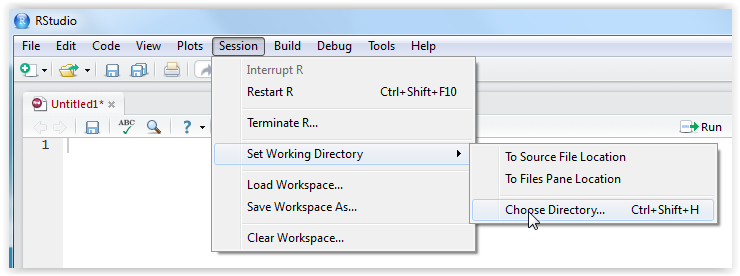
\includegraphics{imgs/R09.PNG}

\textbf{TIP:} If you're new to R or to any of the functions we'll be using, I
strongly encourage you to open a new R script. Copy and paste the R code into
the script, run it to see what happens, and, most importantly, play with it.
Kids learn tons when they play. If you play with the R code, you'll learn tons
too.

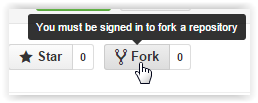
\includegraphics{imgs/R10.PNG}

Now that you're in your assignment directory, enter the following to assign
the data in politics.csv to a variable called politics.

\begin{Schunk}
\begin{Sinput}
> politics<-read.csv("politics.csv")
\end{Sinput}
\end{Schunk}

We can name our variables almost anything we want. We could name the variable
"data,'' ``x,'' or ``my\_awesome\_data.'' ``<-'' is an assignment operator. We
can use it to assign data to variables (e.g. a<-2) or change existing variables.
``read.csv'' is an R function. R functions take the form of the function name
followed by parentheses (e.g. ``function()''). We tell R what data we want to
use the function on and provide R with any special instructions about how to
process the data inside the parentheses. Thus, the previous line tells R to
read the data contained in the politics.csv file in the data directory and
assign it to the variable politics.

\subsection{R: Examining Data}
It's always a good idea to take a look at your data to get a sense of what you're
working with. There are a couple simple ways to take a quick look at what your
variables contain. My favorite is the ``str'' command which will tell you the 
structure of your data.

\begin{Schunk}
\begin{Sinput}
> str(politics)
\end{Sinput}
\begin{Soutput}
'data.frame':	132 obs. of  7 variables:
 $ subject      : int  1 2 3 4 5 6 7 8 9 10 ...
 $ party        : Factor w/ 3 levels "democrat","independent",..: 3 3 2 2 2 3 3 2 3 2 ...
 $ testtime     : Factor w/ 2 levels "post","pre": 2 2 2 2 2 2 2 2 2 2 ...
 $ optimismscore: int  52 51 69 51 61 31 57 48 42 64 ...
 $ minwage      : Factor w/ 2 levels "no","yes": 1 1 2 1 2 1 1 1 1 1 ...
 $ sex          : Factor w/ 2 levels "female","male": 2 2 1 2 2 2 2 2 2 2 ...
 $ income       : num  37.3 42.3 73 33.8 57.3 ...
\end{Soutput}
\end{Schunk}

As you can see, politics is a data frame that has 132 observations of 7 variables.
A data frame is one of several
\href{http://www.statmethods.net/input/datatypes.html}{data types}. The most basic
data type is a vector which is simply a collection of similar variables. These
variables could be numbers (i.e. integers or int), like the subject variable in
the politics data frame. They could also be strings (i.e. text; e.g. ``a,'' ``b,''
and ``c'').

A factor variable is a special type of vector that represents some nominal
(i.e. categorical) data type (e.g. the sex variable that has two levels: male
and female). What distinguishes a vector from a factor is that R treats factors
in a way that will allow us analyze data related to different levels of the
factor.

Each value in a set of data can be accessed by their index
location (i.e. a number that tells you which piece of data you want). Because
a data frame is a two dimensional structure (e.g. it has rows and columns), we
can see what's in any single location by specifying the row and column for the
data frame. Let's see what political affiliation the 5th participant had.

\begin{Schunk}
\begin{Sinput}
> politics[5,2]
\end{Sinput}
\begin{Soutput}
[1] independent
Levels: democrat independent republican
\end{Soutput}
\end{Schunk}

Notice that I told R what data I wanted to use (i.e. politics). Then I provided
R with the row and column (i.e. [5,2]) I was interested in.

If we want to see all the data that are in a particular row, we can specify only
the row we want.

\begin{Schunk}
\begin{Sinput}
> politics[5,]
\end{Sinput}
\begin{Soutput}
  subject       party testtime optimismscore minwage  sex
5       5 independent      pre            61     yes male
    income
5 57.34959
\end{Soutput}
\end{Schunk}

Leaving the column index empty tells R that we want all the values of the 5th row.

Alternatively, if we wanted to see all the data that are in a particular column,
we can specify only that column. Because there's more data than I want to output
here, I'll introduce you to another command (i.e. head), that will show us the 
first several observations from a large data set.

\begin{Schunk}
\begin{Sinput}
> head(politics[,2])
\end{Sinput}
\begin{Soutput}
[1] republican  republican  independent independent
[5] independent republican 
Levels: democrat independent republican
\end{Soutput}
\end{Schunk}

Notice that we just wrapped politics[,2] in another function. We can use this type
of construction to perform functions on only the data we want. Also notice that
I left the row value empty which means you want all the data from the 2nd column.

There's a simpler way to refer to variables within a data frame. Simply name the
data frame, follow it with a dollar sign, and indicate the variable you want.

\begin{Schunk}
\begin{Sinput}
> tail(politics$income)
\end{Sinput}
\begin{Soutput}
[1]  6.054805 52.399731 89.098814 57.707833 17.419496
[6] 23.979241
\end{Soutput}
\end{Schunk}

Unlike head which gives us the first several values, tail will give us the last.
Thus, here we're seeing what the last 6 values in the income column are.

If we wanted to see the 28th income we could say either of the following.
\begin{Schunk}
\begin{Sinput}
> politics[28,7]
\end{Sinput}
\begin{Soutput}
[1] 67.86206
\end{Soutput}
\begin{Sinput}
> politics$income[28]
\end{Sinput}
\begin{Soutput}
[1] 67.86206
\end{Soutput}
\end{Schunk}

I prefer the second construction, because it's easy to accidentally use the
wrong column number. Remembering the variable name is so much easier.

I've shown you that you can get one piece of data by specifying the row and column.
I've also shown you how to get everything from a particular row or column. However,
what if we wanted to get a subset of data from a row or a column? Imagine we
wanted to get all the incomes from the participants. If you look at the politics
data frame, you'll see that each income is represented twice (i.e. once with
the pretest and once with the posttest). How do we get this data?

Certainly we could get each value by itself (e.g. politics\$income[1],
politics\$income[2]...), but that would be incredibly cumbersome. So let me show
you a couple other ways to quickly subset the data.

To subset the data we need to create a vector of the data that we want to get.
Without knowing it we've already created vectors with a single item.

\begin{Schunk}
\begin{Sinput}
> 2
\end{Sinput}
\begin{Soutput}
[1] 2
\end{Soutput}
\end{Schunk}

Notice how after entering 2, R returns ``[1] 2.'' This indicates 2 is a vector.
[1] indicates the index for the adjacent value. There's only one value, so this
vector has a length of one. We can verify this by asking R the length of 2.

\begin{Schunk}
\begin{Sinput}
> length(2)
\end{Sinput}
\begin{Soutput}
[1] 1
\end{Soutput}
\end{Schunk}

There are several ways that we can create vectors. If we want to get the first
66 values, we can create a vector that goes from one to 66 using 1:66. I'm
using head below so the output isn't unreasonably long.

\begin{Schunk}
\begin{Sinput}
> head(1:66)
\end{Sinput}
\begin{Soutput}
[1] 1 2 3 4 5 6
\end{Soutput}
\end{Schunk}

You can also reverse the order (i.e. 66:1) which will create the same vector in
descending order.

Another way of creating a vector is to use the concatenate function (i.e. ``c'').
When you \href{http://www.merriam-webster.com/dictionary/concatenate}{concatenate}
something you link together the things being concatenated. In R this means that
you'll create a vector out of the information that you provide it. 1:3 automatically
concatenates the values 1, 2, and 3. Imagine we wanted to get the first 3 values,
the 12th value, the 61st value, and the last 3 values. length(politics\$income) will
tell us the index of the last observation in income, so we can use this value to
create the vector we want. I'll assign this vector to a variable ``a'' so we
can use this to get the data we want.

\begin{Schunk}
\begin{Sinput}
> a<-c(1:3,12,61,(length(politics$income)-2):length(politics$income))
> politics$income[a]
\end{Sinput}
\begin{Soutput}
[1] 37.280152 42.298008 73.049778 77.556914  6.054805
[6] 57.707833 17.419496 23.979241
\end{Soutput}
\end{Schunk}

``a'' is a vector containing 1 to 3, 12, 61, and 130-132. You could
specify each of these values manually (e.g. ``c(1,2,3,12,61,130,131,132)''), but
I wanted to show you how to minimize how much you're manually entering data.
http://cran.rstudio.com/web/packages/dplyr/vignettes/introduction.html
\textbf{TIP:} If you're not familiar with R's order of operations, make sure you use parentheses
to group the pieces you want together (e.g. ``(length(politics\$income) - 3)'').

To further minimize how much you manually enter data. Applying a bit of logic
can be incredibly helpful. Logic concerns what is true and what is false. R allows
us to use logical expressions to quickly evaluate when some condition is true.
Two of the logical expressions that are particularly useful to subset data are the
equals (i.e. ``=='') and does not equal (i.e. ``!='') operators. We can use them to
determine whether one thing is equal to something else.

\begin{Schunk}
\begin{Sinput}
> 2==2
\end{Sinput}
\begin{Soutput}
[1] TRUE
\end{Soutput}
\begin{Sinput}
> 2==3
\end{Sinput}
\begin{Soutput}
[1] FALSE
\end{Soutput}
\begin{Sinput}
> 2!=3
\end{Sinput}
\begin{Soutput}
[1] TRUE
\end{Soutput}
\end{Schunk}

Let's say we wanted to see which values at the head of politics\$party were
independents. Let's compare the following heads.

\begin{Schunk}
\begin{Sinput}
> head(politics$party)
\end{Sinput}
\begin{Soutput}
[1] republican  republican  independent independent
[5] independent republican 
Levels: democrat independent republican
\end{Soutput}
\begin{Sinput}
> head(politics$party=="independent")
\end{Sinput}
\begin{Soutput}
[1] FALSE FALSE  TRUE  TRUE  TRUE FALSE
\end{Soutput}
\end{Schunk}

You'll see that the second statement creates a vector of
\href{http://en.wikipedia.org/wiki/Boolean}{boolean} (i.e. true or false)
values.

R can handle more complex logical operations by using other
\href{http://astrostatistics.psu.edu/su07/R/html/base/html/Logic.html}
{logical operators}. The logical and (i.e. ``\&'') will tell us when statements
like political party equals Independent \emph{AND} sex doesn't equal
female are true or false.

\begin{Schunk}
\begin{Sinput}
> head((politics$party=="independent")&
+     (politics$sex!="female"))
\end{Sinput}
\begin{Soutput}
[1] FALSE FALSE FALSE  TRUE  TRUE FALSE
\end{Soutput}
\end{Schunk}

Notice how I used parentheses to make it clear which statements went together.
Normally, I would write the entire expression on a single
line. However, due to the margin constraints, I inserted a line break. When
you type enter before you've finished an expression, R will automatically
change the ``>'' prompt to ``+'' so you know you have more to add to finish
the expression. If you ever think you finished an expression and see this,
it's probably a missing close parenthesis, quote, or something else. If you
can't fix the expression, press ``Esc'' to go back to the regular command line.

Although breaking the lines will mean you can see the whole expression, if you
try to copy and paste the expression as is, with the plus signs, you probably
won't get the right answers. So copy and paste the code segments or, better yet,
practice typing them to lay down a better memory trace.

The logical or (i.e. ``|'') will tell us when statements like political party
equals Independent \emph{OR} Republican are true.

\begin{Schunk}
\begin{Sinput}
> head((politics$party=="independent")|
+     (politics$party=="republican"))
\end{Sinput}
\begin{Soutput}
[1] TRUE TRUE TRUE TRUE TRUE TRUE
\end{Soutput}
\end{Schunk}

You can build some very complex statements with logic. I strongly recommend checking
some data you know should be true or false to make sure your code is working the
way you think it should.

The whole point of this was to show you how to select data using logical
expressions. If we have a vector of true false values, we can use that vector
to select only the values associated with the true or false values. Remember,
we only wanted to get the incomes associated with the pretest conditions.
We know the first 66 values were from the pretest, so politics\$income[1:66] would work.
However, imagine that the pre- and posttest
data were mixed up. Rather than manually identifying each row from the pretest,
and massively increasing the chance we make a mistake, we can use a little bit
of logic to get exactly what we need.

\begin{Schunk}
\begin{Sinput}
> head(politics$income[politics$testtime=="pre"])
\end{Sinput}
\begin{Soutput}
[1] 37.28015 42.29801 73.04978 33.82229 57.34959 12.33421
\end{Soutput}
\end{Schunk}

In plain English, this statement says that we want the first six incomes from
the pretests.

\subsection{R: Double Checking Data}
I love running fully computerized experiments because you don't have to manually
enter any data. It's easy to make a mistake when entering data and can be hard
to spot. In graduate school I was the Teaching Assistant for a stats class and
one of the students was so frustrated that they kept getting an assignment back
to redo. The student had checked and double checked the analyses and was
confident that they were correct (they were). Unfortunately, the student had
made some data entry errors. Thus, although the analyses were right, they got
the wrong answers because they were working with the wrong data.

If you're manually entering any data, I strongly suggest doing it twice. If you're
in a group, having everyone enter all the data independently can also be a good
way to go.

Once you have two sets of data, you can compare them. Although I generated the
data so that the second half should correspond to the first half, I haven't yet
checked this. So let's use a bit of logic to compare the data that should be
the same from the first and second halves.

\begin{Schunk}
\begin{Sinput}
> head(politics$subject[politics$testtime=="pre"]==
+     politics$subject[politics$testtime=="post"])
\end{Sinput}
\begin{Soutput}
[1] TRUE TRUE TRUE TRUE TRUE TRUE
\end{Soutput}
\end{Schunk}

Just looking at the head isn't good enough, as there might be FALSE values
somewhere later. If only there were some way to quickly determine how many
false values there were. Fortunately there is. The sum function adds up 
all the values in a vector.

\begin{Schunk}
\begin{Sinput}
> sum(1:3)
\end{Sinput}
\begin{Soutput}
[1] 6
\end{Soutput}
\end{Schunk}

With TRUE and FALSE values, TRUE=1 and FALSE=0.

\begin{Schunk}
\begin{Sinput}
> sum(c(TRUE,TRUE,FALSE,FALSE,FALSE))
\end{Sinput}
\begin{Soutput}
[1] 2
\end{Soutput}
\end{Schunk}

That's all fine and dandy, but we want to see if there are any times the values
are false. If we have a large data set and we see there were 1,382 trues, do
you know if there were any falses? Not without more information.

Just like the exclamation point changes equals to does \emph{not} equal, it can
also be used to change TRUE to FALSE and vice versa. So instead of getting the
sum of TRUE, we want to get the sum of \emph{not} TRUE.

\begin{Schunk}
\begin{Sinput}
> sum(!c(TRUE,TRUE,FALSE,FALSE,FALSE))
\end{Sinput}
\begin{Soutput}
[1] 3
\end{Soutput}
\end{Schunk}

Thus we quickly determine if we've made data entry errors by comparing values
that should be equivalent. To condense the code, I'm going to assign the vector
indicating which values are associated with the pretests to a variable called
trues and use that.

\begin{Schunk}
\begin{Sinput}
> trues<-politics$testtime=="pre"
> sum(!(politics$subject[trues]==politics$subject[!trues]))
\end{Sinput}
\begin{Soutput}
[1] 0
\end{Soutput}
\end{Schunk}

In plain English, we're counting how many of times the subjects in the order
they are during the pretest are in the same order during the posttest. Let's
make sure the other values that should be the same are too.

\begin{Schunk}
\begin{Sinput}
> sum(!(politics$party[trues]==politics$party[!trues]))
\end{Sinput}
\begin{Soutput}
[1] 0
\end{Soutput}
\begin{Sinput}
> sum(!(politics$subject[trues]==politics$subject[!trues]))
\end{Sinput}
\begin{Soutput}
[1] 0
\end{Soutput}
\begin{Sinput}
> sum(!(politics$sex[trues]==politics$sex[!trues]))
\end{Sinput}
\begin{Soutput}
[1] 0
\end{Soutput}
\begin{Sinput}
> sum(!(politics$income[trues]==politics$income[!trues]))
\end{Sinput}
\begin{Soutput}
[1] 0
\end{Soutput}
\end{Schunk}

Sweet! I didn't screw up.

It's also a good idea to check the structure of your data to look for any
abnormalities.

Looking at the structure for politics (see above), I see a couple things I
don't like. First, subject isn't treated as a factor. To fix that, we can
explicitly tell R to change what we have to a factor. We'll factor the subject
variable and assign that back to the subject variable.

\begin{Schunk}
\begin{Sinput}
> politics$subject<-factor(politics$subject)
\end{Sinput}
\end{Schunk}

I don't really care what order the parties, sexes, or minimum wage responses are
in, but I do think the pretests should come before the posttests in the testtime
factor levels. But right now post is first because R alphabetizes the order of
factors unless explicitly told otherwise. Let's fix that now. To fix this, we'll
ask R to refactor the testtime variable with the levels we want, instead of the
levels it automatically chooses.

\begin{Schunk}
\begin{Sinput}
> politics$testtime<-factor(politics$testtime, levels=c("pre", "post"))
\end{Sinput}
\end{Schunk}

We can double check the politics variable to make sure that things are the
way we intended.

\begin{Schunk}
\begin{Sinput}
> str(politics)
\end{Sinput}
\begin{Soutput}
'data.frame':	132 obs. of  7 variables:
 $ subject      : Factor w/ 66 levels "1","2","3","4",..: 1 2 3 4 5 6 7 8 9 10 ...
 $ party        : Factor w/ 3 levels "democrat","independent",..: 3 3 2 2 2 3 3 2 3 2 ...
 $ testtime     : Factor w/ 2 levels "pre","post": 1 1 1 1 1 1 1 1 1 1 ...
 $ optimismscore: int  52 51 69 51 61 31 57 48 42 64 ...
 $ minwage      : Factor w/ 2 levels "no","yes": 1 1 2 1 2 1 1 1 1 1 ...
 $ sex          : Factor w/ 2 levels "female","male": 2 2 1 2 2 2 2 2 2 2 ...
 $ income       : num  37.3 42.3 73 33.8 57.3 ...
\end{Soutput}
\end{Schunk}

Much better!



\subsection{R: Describing Data}
After you've verified your data is correct, you can start describing it. R provides
some sweet tools to help you describe your data. Let's describe the incomes. Because
I have the incomes represented twice in the data frame, I'll assign the incomes from
the pretests to a variable called incomes. Then I show you a great way to quickly
get a sense for your data.

\begin{Schunk}
\begin{Sinput}
> incomes<-politics$income[trues]
> summary(incomes)
\end{Sinput}
\begin{Soutput}
   Min. 1st Qu.  Median    Mean 3rd Qu.    Max. 
  5.672  27.760  41.220  43.040  55.920 114.800 
\end{Soutput}
\end{Schunk}

Here, I'm summarizing the income data. As the income data for each participant were
represented twice, I'm only looking at the pretest data here. You'll see summary
provides the minimum, maximum, 1st quartile, 2nd quartile (i.e. median), 3rd quartile,
and mean. Had you wanted only the minimum, maximum, median, or mean, you could have
used the following functions.

\begin{Schunk}
\begin{Sinput}
> min(incomes)
\end{Sinput}
\begin{Soutput}
[1] 5.672011
\end{Soutput}
\begin{Sinput}
> max(incomes)
\end{Sinput}
\begin{Soutput}
[1] 114.7565
\end{Soutput}
\begin{Sinput}
> median(incomes)
\end{Sinput}
\begin{Soutput}
[1] 41.21894
\end{Soutput}
\begin{Sinput}
> mean(incomes)
\end{Sinput}
\begin{Soutput}
[1] 43.0403
\end{Soutput}
\end{Schunk}

Finding variance and standard deviations are similarly easy.

\begin{Schunk}
\begin{Sinput}
> var(incomes)
\end{Sinput}
\begin{Soutput}
[1] 489.7308
\end{Soutput}
\begin{Sinput}
> sd(incomes)
\end{Sinput}
\begin{Soutput}
[1] 22.12986
\end{Soutput}
\begin{Sinput}
> sd(incomes)==sqrt(var(incomes))
\end{Sinput}
\begin{Soutput}
[1] TRUE
\end{Soutput}
\end{Schunk}

The standard deviation equals the square root of the variance so everything is as it
should be. However, Does the variance represent the unbiased estimate of the population
variance? Let's find out.

\begin{Schunk}
\begin{Sinput}
> biased<-sum((incomes-mean(incomes))^2)/length(incomes)
> unbiased<-sum((incomes-mean(incomes))^2)/(length(incomes)-1)
> var(incomes)==biased
\end{Sinput}
\begin{Soutput}
[1] FALSE
\end{Soutput}
\begin{Sinput}
> var(incomes)==unbiased
\end{Sinput}
\begin{Soutput}
[1] TRUE
\end{Soutput}
\end{Schunk}

Hooray. It's the unbiased estimate. This is good because will use it to calculate
the standard error of the mean.

\begin{Schunk}
\begin{Sinput}
> sem<-sd(incomes)/sqrt(length(incomes))
\end{Sinput}
\end{Schunk}

Sweet. We can use 2.72399776853388 to calculate confidence intervals or make error bars.

Before moving on. Let's take a look at the distribution of incomes using a histogram.

\begin{Schunk}
\begin{Sinput}
> hist(incomes)
\end{Sinput}
\end{Schunk}
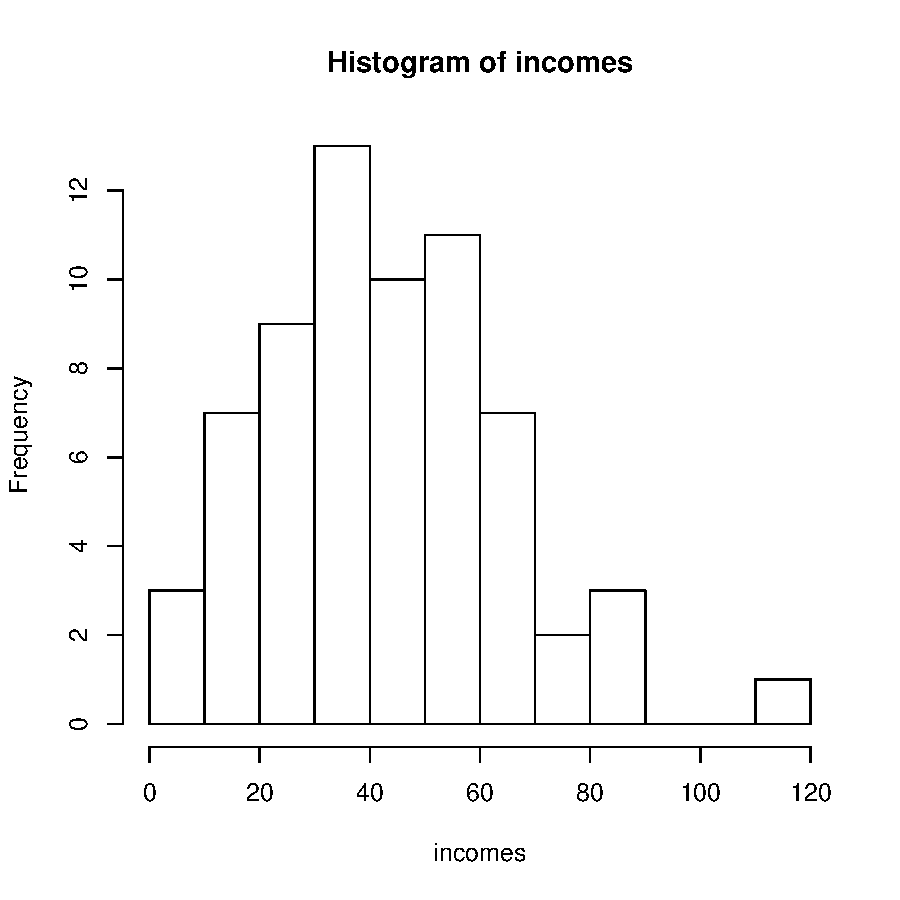
\includegraphics{Reproducibility-033}

Wow, that was ridiculously easy.

\subsection{R: Analyzing Data and Creating Figures}
At this point you should know how to read data, subset data, and create several
highly used descriptive statistics for those data. Now it's time to take what
you already know and see how to run some common analyses, create tables, and
create publication worthy figures using R.

Before we do this, you're going to need to install a couple R packages to make
things easier. To simplify how we subset and summarize data, we're going
to install the package dplyr. To simplify how we work with graphs, we're going
to install ggplot2. We'll also install the package gplots to use some color
commands. Should you be asked whether you want to install additional
packages that are needed for either dplyr or ggplot 2, do it. Should you find
that installing these packages doesn't allow you to follow along. Please shoot
me an email with any error messages ASAP so I can update these instructions.

\begin{Schunk}
\begin{Sinput}
> install.packages("dplyr")
> install.packages("ggplot2")
> install.packages("gplots")
\end{Sinput}
\end{Schunk}

Easy peasy. Now that you have the packages installed, you need to tell R that
you want to work with them.

\begin{Schunk}
\begin{Sinput}
> library("dplyr")
> library("ggplot2")
> library("gplots")
\end{Sinput}
\end{Schunk}

\subsubsection{R: Chi-Square Tests and Tables}
Chi-square tests are used to determine whether two categorical variables
are independent of one another. One question we could ask using the politics
data is whether political affiliation is independent of supporting minimum
wage hikes.

If you remember from statistics, the chi-square test takes the number of
observations for each combination of the categorical variables and compares
that to the number of observations we'd expect for that combination.

Now before we get cracking. I want to reiterate that for each participant I
have their party, income, etc. twice. I don't want to count each observation
twice, so I'm going to split the data.

\begin{Schunk}
\begin{Sinput}
> pre=politics[trues,]
> post=politics[!trues,]
\end{Sinput}
\end{Schunk}

This will give me two data frames. One for the pretest data and one for the
posttest data. As I didn't specify individual columns, all of them will be
in these two data frames.

Ok, lets count the number of observations we have for each combination of the
party and minwage factors. Rather than doing complex formulas involving sums and
logic, we'll use the table function.

\begin{Schunk}
\begin{Sinput}
> mytable<-table(pre$party,pre$minwage)
> mytable
\end{Sinput}
\begin{Soutput}
              no yes
  democrat     8  18
  independent 11   6
  republican  14   9
\end{Soutput}
\end{Schunk}

You can copy and paste the table into Excel or some other spreadsheet to 
create pretty tables with better labels and titles to use in presentations
or publications.

\begin{Schunk}
\begin{Sinput}
> write.table(mytable,"clipboard",sep="\t",col.names=NA)
\end{Sinput}
\end{Schunk}

Ok, so we have the totals. Rather than go through manually and compute the row
and column margins, we can have R do it for us.

\begin{Schunk}
\begin{Sinput}
> margin.table(mytable,1) #Row margins
\end{Sinput}
\begin{Soutput}
   democrat independent  republican 
         26          17          23 
\end{Soutput}
\begin{Sinput}
> margin.table(mytable,2) #Column margins
\end{Sinput}
\begin{Soutput}
 no yes 
 33  33 
\end{Soutput}
\end{Schunk}

We also don't have to compute the expected frequencies long hand. In fact, we
can just tell R what the categorical variables are and it will run the chi-square
test for us.

\begin{Schunk}
\begin{Sinput}
> chisq.test(pre$party,pre$minwage)
\end{Sinput}
\begin{Soutput}
	Pearson's Chi-squared test

data:  pre$party and pre$minwage
X-squared = 6.4037, df = 2, p-value = 0.04069
\end{Soutput}
\end{Schunk}

Sweet. we have everything we need to write up our data. The results of a statistical
test are typically written up in the following format:
\begin{verbatim}
Test name/symbol(degrees of freedom) = test value, p=p-value.
\end{verbatim}

\begin{Schunk}
\begin{Sinput}
> cs<-chisq.test(pre$party,pre$minwage)
\end{Sinput}
\end{Schunk}

Thus we'll have $X^{2}$(2) = 
6.40, p = 
0.041. With this result, we'd reject the
null hypothesis that party affiliation is independent of one's agreement to support
increasing the minimum wage. We could also say that democrats support minimum wage hikes
more than the other parties.

\subsubsection{R: t-tests and Bar Graphs}
Let's say we wanted to see if there was a difference in how optimistic males and females
were before the manipulation. To test the null hypothesis that there is no difference,
we can run a t-test. Hopefully, you remember that there are different types of t-tests.
As males and females represent different groups of people we'll need to use an
independent t-test.

There are a couple ways we can go about doing this. First we'll take use the
way you should be fairly familiar with.

\begin{Schunk}
\begin{Sinput}
> t.test(pre$optimism[pre$sex=="male"],
+        pre$optimism[pre$sex=="female"],
+        paired=FALSE, var.equal=FALSE,
+        alternative="two.sided",
+        conf.level=.95)
\end{Sinput}
\begin{Soutput}
	Welch Two Sample t-test

data:  pre$optimism[pre$sex == "male"] and pre$optimism[pre$sex == "female"]
t = -0.3744, df = 62.936, p-value = 0.7094
alternative hypothesis: true difference in means is not equal to 0
95 percent confidence interval:
 -10.946279   7.491733
sample estimates:
mean of x mean of y 
 54.12121  55.84848 
\end{Soutput}
\end{Schunk}

As you can see from the output, males and females didn't differ in terms of their optimism
t(62.94) = -.37, p = .71.

The first two arguments that we passed to the function t.test were the data we wanted to
compare. Here we were comparing optimism scores for males and optimism scores for
females. The other arguments are the defaults, so we didn't have to include them. I
included them to show you how to change the type of test you're doing. ``paired=FALSE'' tells
R that we want to run an independent t-test. If we wanted to run an independent t-test
we'd say TRUE. ``var.equal=FALSE'' tells R that we don't want to assume the variances
are equal. You should use this unless you test and fail to reject the null hypothesis
that they are equal. ``alternative'' is used to indicate what alternative hypothesis is.
If it's that there's difference without predicting a direction, use ``two.sided.''
If the alternative states that the first set (e.g. males in this example) is greater
than the second, use ``greater.'' If the alternative states the first set is less than
the second, use ``less.'' Finally, the conf.level determines the alpha level for your
test. Set conf.level to 1-alpha.

Let's pretend you ran a 2-way mixed ANOVA on the optimism scores from politics
data set with party and as the between-subjects factor and testtime as the within-subjects
factor using the subject factor in the error term (I'll show you how to do this later).
Imagine you found a significant interaction between party and testtime which indicates
that individuals from different parties were differentially affected by watching the
videos. You want to run some post-hoc tests to determine whether or not the difference
between pre- and posttests for Republicans was significant. Because testtime is a
within-subjects variable, we can run a paired t-test. Let's also use a Bonferroni correction
on the t-test so we don't artificially increase our alpha level.

\begin{Schunk}
\begin{Sinput}
> t.test(politics$optimism[(politics$testtime=="pre")&
+                         (politics$party=="republican")],
+        politics$optimism[(politics$testtime=="post")&
+                         (politics$party=="republican")],
+        paired=TRUE, conf.level=1-.05/3)
\end{Sinput}
\begin{Soutput}
	Paired t-test

data:  politics$optimism[(politics$testtime == "pre") & (politics$party ==  and politics$optimism[(politics$testtime == "post") & (politics$party ==     "republican")] and     "republican")]
t = -4.5325, df = 22, p-value = 0.0001643
alternative hypothesis: true difference in means is not equal to 0
98.33333 percent confidence interval:
 -10.31856  -2.81187
sample estimates:
mean of the differences 
              -6.565217 
\end{Soutput}
\end{Schunk}

Republicans were more optimistic after watching the videos t(22) = -4.53,
p < .001. Since we have a significant difference, we might want to create
a figure to quickly summarize the results. We'll use a bar graph as the
independent variable is categorical (i.e. pre- or posttest). To create the
graph, we'll need to calculate the means and standard errors of the means
for the pre- and post-tests for the republicans.

Although calculating means and standard errors for two groups can be
simply accomplished using the functions mean, sd, and sqrt with a bit
of logic. I'd like to show you another way that will pay off handsomely
when you have a lot of different conditions. To follow the example, you
need to have the dplyr, ggplot2, and gplots libraries installed and loaded.

We'll be making heavy use of the ``\%>\%'' operator which allows us to chain a series
of operations together. We've already chained functions together by nesting functions
(e.g. mean(head(politics\$optimismscore))), but using the \%>\% will provide us a more
elegant way of getting the information we need in a way that we can easily use in creating
figures.

What we're going to do is take the politics dataset and group it by testtime and party.
We'll then calculate the means and standard errors of the means of the optimism scores
for the different conditions.


\begin{Schunk}
\begin{Sinput}
> polsum<-politics%>%group_by(party,testtime)%>%arrange(party,testtime)%>%
+     summarize(means=mean(optimismscore),
+               sems=sd(optimismscore)/sqrt(length(optimismscore)))
\end{Sinput}
\end{Schunk}

dplyr is fairly intelligent. After specifying politics, it knows that's the data frame
we're going to work with. Thus, we don't have to create long and windy expressions like
``group\_by(politics\$party).'' In plain English, the statement says that we're going to
work with the politics data
frame. We're going to group it by party and testtime which will create each combination
of the levels of party and testtime as separate conditions which will appear in different
rows. Then for each condition, we're going to calculate the means of all the optimism
scores in that group and assign it to the variable means. We're doing the same thing
to calculate the standard errors of the means and assigning it to the variable sems.
We'll take the output of these operations and assign it to a variable called polsum,
which is short for \emph{pol}itics \emph{sum}mary. Let's see what polsum looks like.

\begin{Schunk}
\begin{Sinput}
> polsum
\end{Sinput}
\begin{Soutput}
Source: local data frame [6 x 4]
Groups: party

        party testtime    means     sems
1    democrat      pre 70.23077 2.502496
2    democrat     post 74.26923 2.600922
3 independent      pre 53.05882 2.706841
4 independent     post 56.76471 2.200484
5  republican      pre 39.17391 3.016196
6  republican     post 45.73913 3.442479
\end{Soutput}
\end{Schunk}

For the figure that corresponds to the earlier t-test, we only need the data from the
republicans. Let's get that and assign it to a new variable to make additional steps
more clear.

\begin{Schunk}
\begin{Sinput}
> pubs<-polsum[polsum$party=="republican",]
> pubs
\end{Sinput}
\begin{Soutput}
Source: local data frame [2 x 4]
Groups: party

       party testtime    means     sems
1 republican      pre 39.17391 3.016196
2 republican     post 45.73913 3.442479
\end{Soutput}
\end{Schunk}

Groovy. Now let's create a figure. Like most things in R, there are multiple ways to
do the same thing. After having created graphs for years using the standard graphics
package, ggplot2 was like a breath of fresh air. ggplot2 builds up figures in layers
that can be altered and changed to your liking. We'll start with the basic plot and
then make some changes.

\begin{Schunk}
\begin{Sinput}
> fig<-ggplot(pubs,aes(x=factor(testtime),y=means))
> fig<-fig + geom_bar(stat="identity", color="black",
+                     fill=c("deepskyblue2","deeppink"))
\end{Sinput}
\end{Schunk}

The first line tells R to create a ggplot using the pubs data. ``aes'' is short for aesthetic,
which tells ggplot2 roughly how we want the figure to look. We're plotting the factor
testtime on the x axis and the means on the y axis. ``means'' here is the variable in the
pubs data set, not the name of a function.

The second line says that we want to add information to the plot we assigned to the variable
``fig.'' ``fig<-fig+stuff'' means that we're going to take what's already in fig, add some
stuff and assign the result to fig. By using this type of construction, we can build up
fig piece by piece to look exactly how we want it.

Let's add in our error bars that represent one standard error of the mean above and below
each mean. Then we'll take a peek at what we have.
\begin{Schunk}
\begin{Sinput}
> fig<-fig+geom_errorbar(aes(ymax=means+sems, ymin=means-sems), width=.2)
> fig
\end{Sinput}
\end{Schunk}
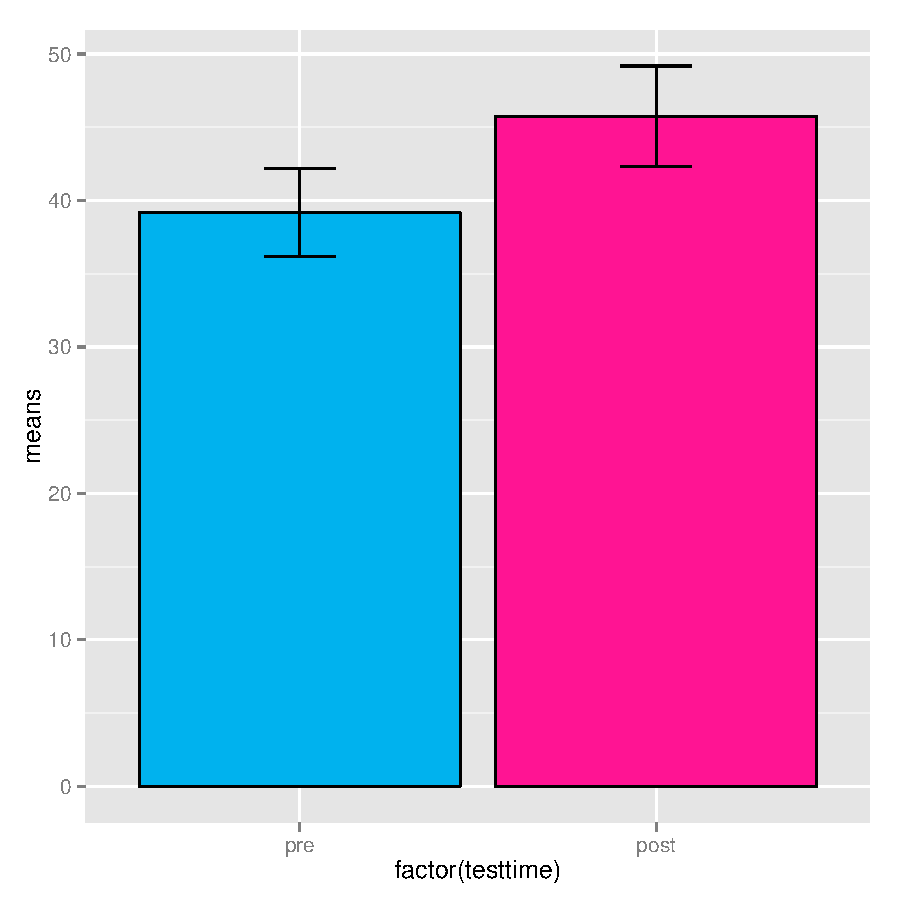
\includegraphics{Reproducibility-048}

Let's give the figure a meaningful title. \textbf{NOTE:} I'm going to show you the commands
one by one, but I won't replot the figure until we're finished. If you want to take a look at
what the figure looks like after any of the steps, type ``fig'' in the console after you make
a change.

\begin{Schunk}
\begin{Sinput}
> fig<-fig+ggtitle("Pre & Post Video Optimism Scores")
\end{Sinput}
\end{Schunk}

Let's change the axis labels.
\begin{Schunk}
\begin{Sinput}
> fig<-fig+labs(x="Test Version", y="Optimism Scores\n(higher=more optimistic")
> fig<-fig+scale_x_discrete(breaks=c("pre","post"),labels=c("Pre","Post"))
\end{Sinput}
\end{Schunk}

Let's change the title size, font, and vertical adjustment.
\begin{Schunk}
\begin{Sinput}
> fig<-fig+theme(plot.title=element_text(size=15,face="bold",vjust=.5))
\end{Sinput}
\end{Schunk}

Let's do the same thing for the axis labels and text.
\begin{Schunk}
\begin{Sinput}
> fig<-fig+theme(axis.title.x=element_text(size=12,face="bold",vjust=-.25))
> fig<-fig+theme(axis.title.y=element_text(size=12,face="bold",vjust=1))
> fig<-fig+theme(axis.text.x=element_text(size=10,face="bold",color="black"))
> fig<-fig+theme(axis.text.y=element_text(size=10,face="bold",color="black"))
\end{Sinput}
\end{Schunk}

Let's change the limits of the y-axis so we can clearly see the effects. I picked
values that would contain the means plus and minus the standard error of the means.
\begin{Schunk}
\begin{Sinput}
> fig<-fig+coord_cartesian(ylim=c(min(pubs$means)-2*max(pubs$sems),
+                                 max(pubs$means)+2*max(pubs$sems)))
\end{Sinput}
\end{Schunk}

Let's make the axes look a little prettier.
\begin{Schunk}
\begin{Sinput}
> fig<-fig+theme(panel.border=element_blank(), axis.line=element_line())
\end{Sinput}
\end{Schunk}

Let's clean up that ugly grey grid and see what we have now.
\begin{Schunk}
\begin{Sinput}
> fig<-fig+theme(panel.grid.major.x=element_blank())
> fig<-fig+theme(panel.grid.major.y=element_line(color="darkgrey"))
> fig<-fig+theme(panel.grid.minor.y=element_blank())
> fig
\end{Sinput}
\end{Schunk}
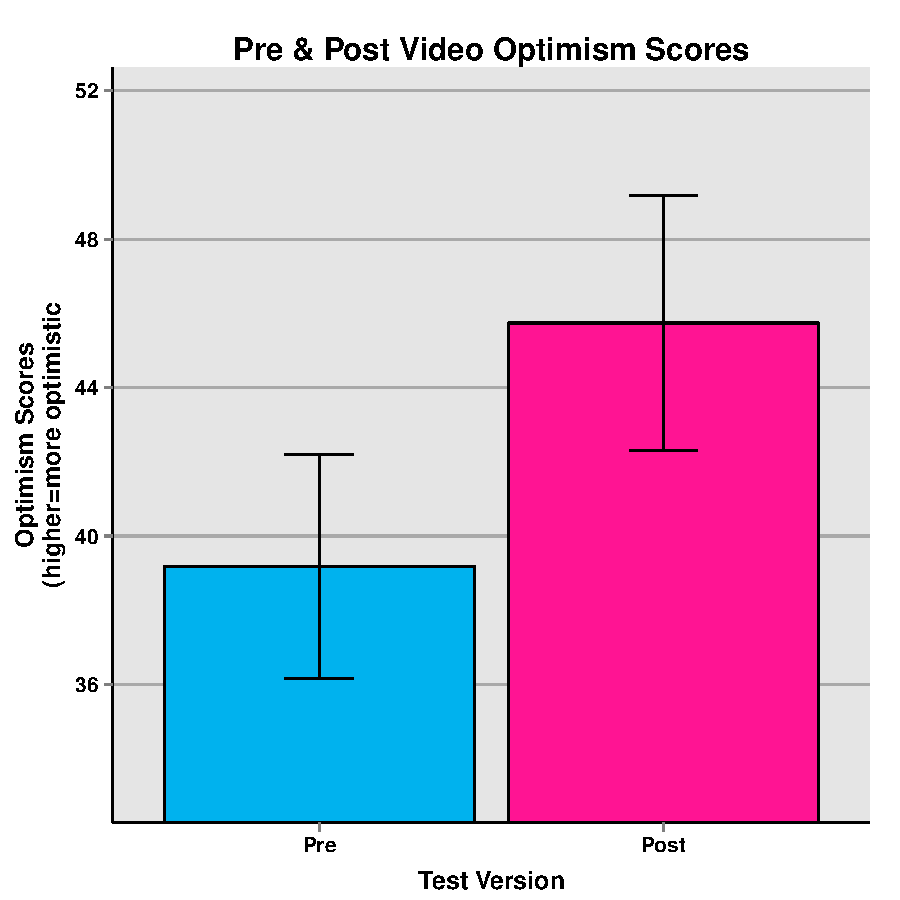
\includegraphics{Reproducibility-055}

Sweet. That looks pretty nice. I highly recommend playing with the different
statements and changing parameters to see what the effect are. Remember, help
can be your friend.

\subsubsection{R: ANOVAs, Grouped Bar Graphs, and Line Graphs}
t-tests are useful when you have a single independent variable with only two
levels. What happens if you have a single independent variable with more
than two levels or more than one independent variable with discrete levels?
ANOVA to the rescue. In this section, we'll take a look at One-way ANOVAs (i.e.
one variable) and multi-way ANOVAs (i.e. more than one variable). We'll
also take a look at performing ANOVAs for within-, between-, and mixed-subjects
designs.

\subsubsubsection{One-Way Between-Subjects ANOVA}
In a between-subjects ANOVA, all the data are coming from different participants.
For the politics dataset, this must be sex, party, or income, as we have multiple
measures of optimism scores. Sex and party are both discrete variables so one
of those will serve as a factor in a one-way ANOVA. As we could just run a t-test
for the sex factor, we'll use party as our independent variable to predict
income. We don't want to inflate our sample size, so we'll only use the politics
data for the pretest.

To run an ANOVA in R, you need to specify your model. A model describes what
effects and interactions you believe explains data. A model will also describe
what will serve as the error term. The error term is really easy for within-subjects
designs, but we'll have to pay attention later so we get the right error terms.

In R, we build a model in the following way.

\begin{verbatim}
DV ~ IV1 + IV2 + ... + Error Terms
\end{verbatim}

The first term represents our dependent variable. The ``~''can be interpreted as
``depends on,'' ``is predicted by,'' or ``is a function of.'' Next we include all
the independent variables we believe predict or affect the dependent variable.
Finally, we specify the error terms when there are different errors for different
effects or interactions. In plain English, the previous statement can be read as
``the dependent variable depends on the effects of different IVs and random error.''
Because there's only a single error term for completely
between-subjects designs, we don't need to worry about the error term yet.

Since our alternative hypothesis here would be that income depends on political
affiliation. This is a very simple model. To run the ANOVA, we provide R the model,
and the data the model represents. We're going to wrap the ANOVA function (aov) in
the summary function as the results from aov won't be very useful by themselves.
Remember we don't want to include the parties and incomes twice!

\begin{Schunk}
\begin{Sinput}
> summary(aov(income~party,data=politics[politics$testtime=="pre",]))
\end{Sinput}
\begin{Soutput}
            Df Sum Sq Mean Sq F value Pr(>F)  
party        2   3973  1986.7   4.493  0.015 *
Residuals   63  27859   442.2                 
---
Signif. codes:  
0 '***' 0.001 '**' 0.01 '*' 0.05 '.' 0.1 ' ' 1
\end{Soutput}
\end{Schunk}

From these results, we would be justified in concluding that income is associated
with political affiliation, F(2, 63) = 4.49, p = .015. Unlike the Chi-square test
and t-tests, there are degrees of freedom for the effect and for the errors (i.e.
residuals). We represent these two types of degrees of freedom using this convention:
F(df-Effect, df-Error).

\subsubsubsection{Two-Way Between-Subjects ANOVA and Grouped Bar Graph}
When we have more than one between-subjects independent variables that are discrete in
nature or measurement, we can use 1-, 2-, ..., n-way ANOVAs. When we have more
than a single variable, we can also observe interactions between the independent
variables. As the number of interactions gets rather large as we add variables,
specifying all the effects and interactions that the dependent variable depends on
can be cumbersome. However, if we specify our model in the following way R will
automatically generate all the interactions of the specified predictors.

\begin{verbatim}
DV ~ IV1 * IV2 * ... + Error Terms
\end{verbatim}

The only difference between the models is that we'd have to specify each independent variable and
each interaction using the ``+'' construction. The ``*'' construction allows us to
specify only the independent variables and the interactions are calculated automatically.

Let's run a 2-way between-subjects ANOVA predicting income from party affiliation and sex.

\begin{Schunk}
\begin{Sinput}
> summary(aov(income~party*sex,data=politics[politics$testtime=="pre",]))
\end{Sinput}
\begin{Soutput}
            Df Sum Sq Mean Sq F value Pr(>F)  
party        2   3973  1986.7   4.544 0.0145 *
sex          1   1563  1563.0   3.575 0.0635 .
party:sex    2     63    31.3   0.072 0.9311  
Residuals   60  26234   437.2                 
---
Signif. codes:  
0 '***' 0.001 '**' 0.01 '*' 0.05 '.' 0.1 ' ' 1
\end{Soutput}
\end{Schunk}

From these results, we would be justified in concluding that income is associated with
political affiliation, F(2, 60) = 4.54, p = .015. Income is not associated with sex, F(1, 60)
= 3.58, p = .064. Additionally there was no interaction between political affiliation and
sex, F(2, 60) = .07, p = .931.

Although I normally wouldn't plot a 2-way interaction that isn't significant, I'll do it
here anyways so you can see how to create a grouped bar graph. Most of the commands we'll
issue to create the figure should be familiar, so I'll present them all at once. Also,
instead of issuing each command as fig<-fig+stuff, I'm just going to keep adding
everything to the original call to ggplot---there are multiple ways to accomplish the same
effect. After finishing the graph, we'll take a look at it and I'll go over some of the
commands that aren't as familiar. But first I need to use dplyr to summarize the grouped data.


\begin{Schunk}
\begin{Sinput}
> polsum<-politics[politics$testtime=="pre",]%>%group_by(party,sex)%>%
+     summarize(means=mean(income),sems=sd(income)/sqrt(length(income)))
> col1=col2hex("deeppink")
> col2=col2hex("deepskyblue2")
> fig<-ggplot(polsum, aes(x=party, y=means, fill=sex))+
+ geom_bar(stat="identity",position=position_dodge())+
+ scale_fill_manual(values=c(col1,col2),name="Sex",breaks=c("female","male"),
+                   labels=c("Female", "Male"))+
+ theme(legend.key=element_rect(color="black"))+
+ geom_errorbar(aes(ymax=means+sems, ymin=means-sems),
+               width=.2,position=position_dodge(.9))+
+ ggtitle("Incomes by Sex and Political Affiliation")+
+ labs(x="Political Party Affiliation",y="Income\n(thousands of dollars)")+
+ scale_x_discrete(breaks=c("democrat","independent","republican"),
+                  labels=c("Democrat","Independent","Republican"))+
+ theme(plot.title=element_text(size=15,face="bold",vjust=.5))+
+ theme(axis.title.x=element_text(size=12,face="bold",vjust=-.25))+
+ theme(axis.title.y=element_text(size=12,face="bold",vjust=1))+
+ theme(axis.text.x=element_text(size=10,face="bold",color="black"))+
+ theme(axis.text.y=element_text(size=10,face="bold",color="black"))+
+ coord_cartesian(ylim=c(min(polsum$means)-2*max(polsum$sems),
+                       max(polsum$means)+2*max(polsum$sems)))+
+ theme(panel.border=element_blank(),axis.line=element_line())+
+ theme(panel.grid.major.x=element_blank())+
+ theme(panel.grid.major.y=element_line(color="darkgrey"))+
+ theme(panel.grid.minor.y=element_blank())+
+ theme(legend.position=c(.2,.76))+
+ theme(legend.background=element_blank())+
+ theme(legend.background=element_rect(color="black"))+
+ theme(legend.title=element_blank())+
+ theme(legend.title=element_text(size=12))+
+ theme(legend.title.align=.5)+
+ theme(legend.text=element_text(size=10,face="bold"))
> fig
\end{Sinput}
\end{Schunk}
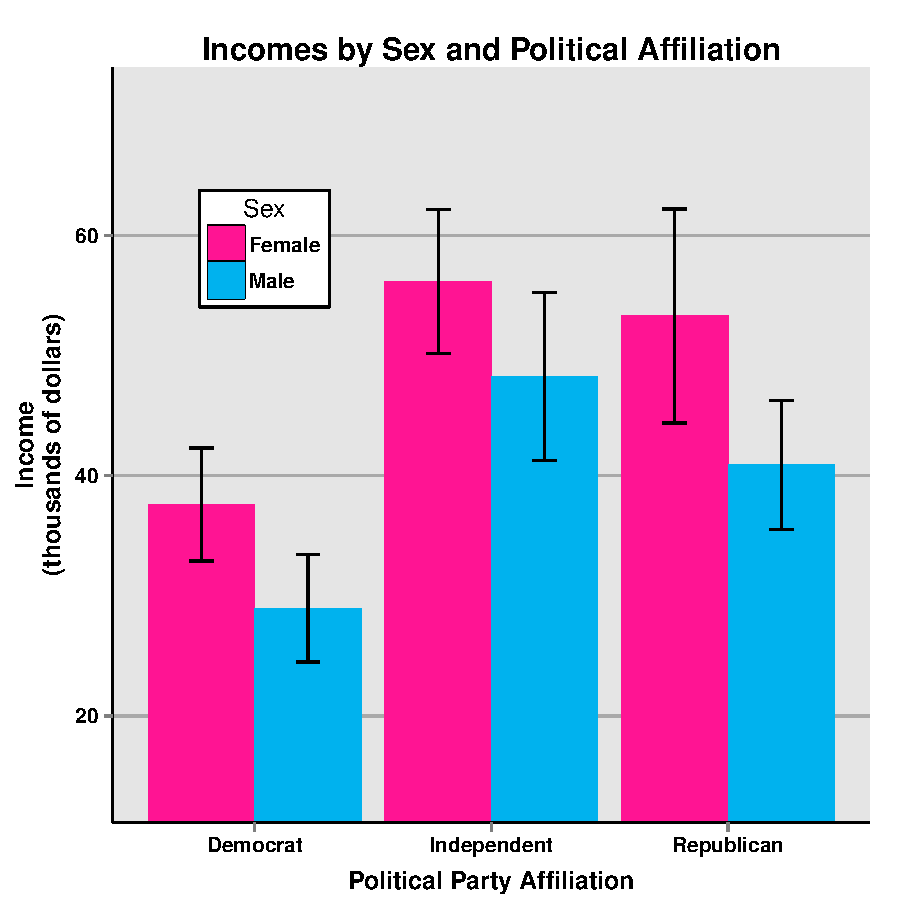
\includegraphics{Reproducibility-058}

I'd encourage you to run through this code piece by piece using the fig<-fig+
construction to see what the different commands do. But here are the most
important differences between this grouped bar graph and the earlier bar graph.
In the original call to ggplot2, I said fill=sex so that the fill was associated
with the different levels of sex. I also manually set the colors I wanted.
Males were ``deepskyblue2'' and females were ``deeppink.'' I saved these color
values before I called ggplot2 to conserve on space so I didn't exceed the margins
for this document by too much.

When specifying that this was a bar graph using ``geom\_bar'' I set position to
position\_dodge. Without doing this, the bars would be stacked on one another
and make any differences harder to visualize. Because of this, I also needed to
dodge the positions of the error bars. I made a second call to ``geom\_bar'' to
avoid having an ugly legend.

Speaking of the legend, when there is more than a single independent variable,
legends are traditionally used to indicate the values of any IVs in the figure
that aren't labeled on the x-axis. All of the commands with ``legend'' or ``guide''
in the arguments work to create, alter, and move the legend.

That's basically it. Although this is a bit more complex than it needs to be just
to create a figure, these commands can make your figure look way better than what
you could easily create using a spreadsheet. Consider my code as a guide when you
create your own figures. Copy, paste, and edit the code when you're creating your
own figures.

\subsubsubsection{Line Graph}
\textbf{WARNING:} You should only create a line graph for a interval or ratio
scale variable. Lines indicate continuity. If you're using a categorical or
ordinal scale variable, you don't have continuity. One caveat, you might have
a ratio scale variable that you have discretely manipulated (e.g. milligrams
of caffeine intake). You can still use a line graph in cases like this.

With that warning in mind, I'm creating a line graph for the data we used
previously as an example for how to create line graphs.

It's probably no surprise that instead of using ``geom\_bar,'' we'll now be using
``geom\_line.'' I'll also be using ``geom\_point'' to make points to represent the
means we observed. All the differences between this figure and the previous one
are contained in the first 5 lines.

\begin{Schunk}
\begin{Sinput}
> fig<-ggplot(polsum, aes(x=party, y=means, group=sex, color=sex))+
+ geom_line(size=1)+
+ geom_point(size=2)+
+ scale_color_manual(values=c(col1,col2),name="Sex",breaks=c("female","male"),
+                   labels=c("Female", "Male"))+
+ geom_errorbar(aes(ymax=means+sems, ymin=means-sems),width=.2)+
+ ggtitle("Incomes by Sex and Political Affiliation")+
+ labs(x="Political Party Affiliation",y="Income\n(thousands of dollars)")+
+ scale_x_discrete(breaks=c("democrat","independent","republican"),
+                  labels=c("Democrat","Independent","Republican"))+
+ theme(plot.title=element_text(size=15,face="bold",vjust=.5))+
+ theme(axis.title.x=element_text(size=12,face="bold",vjust=-.25))+
+ theme(axis.title.y=element_text(size=12,face="bold",vjust=1))+
+ theme(axis.text.x=element_text(size=10,face="bold",color="black"))+
+ theme(axis.text.y=element_text(size=10,face="bold",color="black"))+
+ coord_cartesian(ylim=c(min(polsum$means)-2*max(polsum$sems),
+                       max(polsum$means)+2*max(polsum$sems)))+
+ theme(panel.border=element_blank(),axis.line=element_line())+
+ theme(panel.grid.major.x=element_blank())+
+ theme(panel.grid.major.y=element_line(color="darkgrey"))+
+ theme(panel.grid.minor.y=element_blank())+
+ theme(legend.position=c(.2,.76))+
+ theme(legend.background=element_blank())+
+ theme(legend.background=element_rect(color="black"))+
+ theme(legend.title=element_blank())+
+ theme(legend.title=element_text(size=12))+
+ theme(legend.title.align=.5)+
+ theme(legend.text=element_text(size=10,face="bold"))
> fig
\end{Sinput}
\end{Schunk}
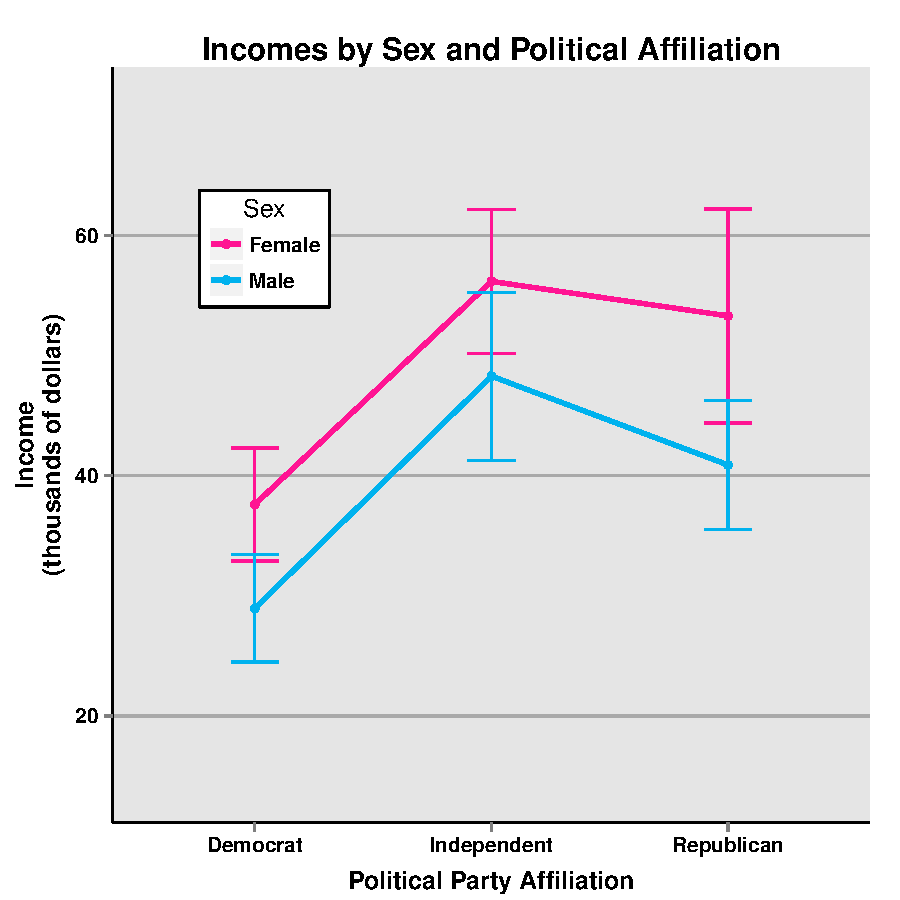
\includegraphics{Reproducibility-059}

In a repeated measures ANOVA, you're observing some variable several times for
each subject (e.g. participant, school, whatever). Thus a repeated measures
design indicates that at least one of the variables
posttest) with 

\subsubsubsection{Within-Subjects ANOVAs}
When you measure a dependent variable several times for each participant and
have more than a single level, you can't use a paired t-test. Instead, you
can use a within-subjects ANOVA. In our politics data set, we observed measured
optimism in pre- and postests with our manipulation falling in between. For
this simple design, we could use a paired test. But let's imagine if there
were three observations after different manipulations.

The whole reason people use within-subjects designs is because they're so much
more powerful than their between-subjects counterparts. They can't always
be used, but when they can they should be. Why are they so powerful? Because
they allow us to break up error variance into multiple pieces. Our earlier
ANOVAs broke variance up into pieces. Pieces related to sex, party, an interaction
between sex and party, and error (i.e. residuals). These residuals can be due
to individual differences, differences in time of day, differences in temperature,
whatever. If we can break up these residuals we can use them to account for some
of these differences.

When we have subjects participating at multiple times, we can attribute some of
this residual variance to the subjects, interactions between the subjects and 
the variables, and interactions between the subjects and interactions of the
variables. Although a full understanding of how this is accomplished is beyond
the scope of this course, R knows how to break up the residuals appropriately
if we specify the appropriate error term.

First, let's analyze the pre- and posttest optimism data as if the data were
from a fully between subjects design. Then we'll analyze the same data with
an appropriate error term and see how that affects things.

\begin{Schunk}
\begin{Sinput}
> summary(aov(optimismscore~testtime, data=politics))
\end{Sinput}
\begin{Soutput}
             Df Sum Sq Mean Sq F value Pr(>F)
testtime      1    771   770.9   2.258  0.135
Residuals   130  44381   341.4               
\end{Soutput}
\end{Schunk}

Based on these results, we'd be justified in concluding that watching the videos
had no effect on optimism scores, F(1, 130) = 2.26, p = .135.

To specify the error term we'll use the following template.

\begin{verbatim}
Error(SubjectVariable/(Within*Subjects*Variables))
\end{verbatim}

``Error'' tells R that the equation that follows will be used for the error terms.
In what follows, we're saying that we want error terms related to the subject variable
for each of the within-subjects variables and their interaction. For this first
example, the error term is really simple.

\begin{Schunk}
\begin{Sinput}
> summary(aov(optimismscore~testtime+Error(subject/testtime),data=politics))
\end{Sinput}
\begin{Soutput}
Error: subject
          Df Sum Sq Mean Sq F value Pr(>F)
Residuals 65  43185   664.4               

Error: subject:testtime
          Df Sum Sq Mean Sq F value   Pr(>F)    
testtime   1  770.9   770.9   41.91 1.46e-08 ***
Residuals 65 1195.6    18.4                     
---
Signif. codes:  
0 '***' 0.001 '**' 0.01 '*' 0.05 '.' 0.1 ' ' 1
\end{Soutput}
\end{Schunk}

\textbf{WARNING:} Remember how earlier, we changed subjects into a factor. If you didn't
do this you didn't get the same output that I did.

If you did everything right you would be justified in concluding that watching
the videos increased optimism scores, F=(1,65), 41.91, p < .001.

Notice how the error has been broken into pieces for the subjects and the interaction
between subjects and testtime. By accounting for variations in individual participants,
we were able to see that the effect of testtime (i.e. exposure to funny videos) was
indeed significant.

For this simple example, we can verify that our results are right with a t-test.

\begin{Schunk}
\begin{Sinput}
> t.test(politics$optimismscore[politics$testtime=="pre"],
+        politics$optimismscore[politics$testtime=="post"],
+        paired=TRUE)
\end{Sinput}
\begin{Soutput}
	Paired t-test

data:  politics$optimismscore[politics$testtime == "pre"] and politics$optimismscore[politics$testtime == "post"]
t = -6.474, df = 65, p-value = 1.458e-08
alternative hypothesis: true difference in means is not equal to 0
95 percent confidence interval:
 -6.324356 -3.342310
sample estimates:
mean of the differences 
              -4.833333 
\end{Soutput}
\end{Schunk}

Notice that the p-value is exactly the same. Yahoo!

\subsubsubsection{Mixed ANOVAs}
When one or more of your variables is within-subjects \emph{AND} one or more of your variables
is between-subjects, you'll have to use a mixed ANOVA. We create our models and error terms
in the same way we did before (represented differently for clarity).

\begin{verbatim}
DV ~ All * The * IVs + Error(SubjectVariable/(Only*The*Within*Subjects*IVs))
\end{verbatim}

The within-subjects ANOVA is just a special case of this general form as all the IVs are
within-subjects IVs. So let's see if pre- posttest optimism scores differed depending on
political party.

\begin{Schunk}
\begin{Sinput}
> summary(aov(optimismscore~testtime*party+Error(subject/testtime),data=politics))
\end{Sinput}
\begin{Soutput}
Error: subject
          Df Sum Sq Mean Sq F value   Pr(>F)    
party      2  21950   10975   32.56 1.95e-10 ***
Residuals 63  21235     337                     
---
Signif. codes:  
0 '***' 0.001 '**' 0.01 '*' 0.05 '.' 0.1 ' ' 1

Error: subject:testtime
               Df Sum Sq Mean Sq F value   Pr(>F)    
testtime        1  770.9   770.9  42.526 1.35e-08 ***
testtime:party  2   53.5    26.8   1.476    0.236    
Residuals      63 1142.1    18.1                     
---
Signif. codes:  
0 '***' 0.001 '**' 0.01 '*' 0.05 '.' 0.1 ' ' 1
\end{Soutput}
\end{Schunk}

From these results, we can conclude that optimism was related to their party affiliation, 
F(2, 63) = 32.56, p < .001. Notice how I said it was related, not it depended on party
affiliation. Since this party affiliation wasn't manipulated, we have to be very cautious
about making claims of causation. Remember correlation $\neq$ causation. We can
also conclude that watching videos did affect optimism, F(1, 63) = 42.53, p < .001. We can
also conclude that watching videos didn't affect individuals with different party affiliations
differently, F(2, 63) = 1.48, p = .236.

\subsubsubsection{Correlation and Simple Regression}
We were justified in using ANOVAs and t-tests in our earlier analyses because the independent
variables had discrete levels (e.g. republican, independent, and democrat). If we wanted
to see whether there was a relationship between two variables that weren't discrete in nature,
we'd need to perform a correlation or regression analysis.

Let's see if incomes were related to optimism pre-scores.

\begin{Schunk}
\begin{Sinput}
> x<-politics$income[politics$testtime=="pre"]
> y<-politics$optimism[politics$testtime=="pre"]
> thecor<-cor(x,y)
> thecor
\end{Sinput}
\begin{Soutput}
[1] -0.09670988
\end{Soutput}
\end{Schunk}

Ok so r=-.097. This suggests a weak negative correlation between income and optimism (i.e. as
income goes up, optimism slightly tends to go down). But we need to run a test to see if
this correlation is significant.

\begin{Schunk}
\begin{Sinput}
> cor.test(x,y)
\end{Sinput}
\begin{Soutput}
	Pearson's product-moment correlation

data:  x and y
t = -0.7773, df = 64, p-value = 0.4398
alternative hypothesis: true correlation is not equal to 0
95 percent confidence interval:
 -0.3309951  0.1488060
sample estimates:
        cor 
-0.09670988 
\end{Soutput}
\end{Schunk}

Based on the results, we should conclude that income and optimism are unrelated, r = -.097,
t(64) = -.78, p = .440. Let's say we found a significant correlation and wanted to create a model
of our data (i.e. the line of best fit). A line needs a slope and an intercept. We could
calculate these using the appropriate formulas.

\begin{Schunk}
\begin{Sinput}
> slope<-thecor*(sd(y)/sd(x))
> intercept<-mean(y)-slope*mean(x)
> slope
\end{Sinput}
\begin{Soutput}
[1] -0.08134829
\end{Soutput}
\begin{Sinput}
> intercept
\end{Sinput}
\begin{Soutput}
[1] 58.4861
\end{Soutput}
\end{Schunk}

Remember, it's not significant, but if it were, this would mean that for each additional
thousand dollars of income, pretest optimism decreased less than 1/10th of a point.

If we know what we want our model to be, we can specify this. Notice how we computed a
slope and an intercept. That's the formula for a line. Thus regression, which seeks to
determine how much the predicted variable changes with changes in the predictor, creates
a linear model. We can build our model like we did earlier models and ask R to summarize
our model which will provide us all the relevant statistics we need.

\begin{Schunk}
\begin{Sinput}
> summary(lm(y~x))
\end{Sinput}
\begin{Soutput}
Call:
lm(formula = y ~ x)

Residuals:
    Min      1Q  Median      3Q     Max 
-38.563 -15.240   1.823  12.637  39.088 

Coefficients:
            Estimate Std. Error t value Pr(>|t|)    
(Intercept) 58.48610    5.05673  11.566   <2e-16 ***
x           -0.08135    0.10465  -0.777     0.44    
---
Signif. codes:  
0 '***' 0.001 '**' 0.01 '*' 0.05 '.' 0.1 ' ' 1

Residual standard error: 18.67 on 64 degrees of freedom
Multiple R-squared:  0.009353,	Adjusted R-squared:  -0.006126 
F-statistic: 0.6042 on 1 and 64 DF,  p-value: 0.4398
\end{Soutput}
\end{Schunk}

Notice this one call gave us $R^2$ which tells you the percent of variance in y that the
model explains. You might notice that this is just the value of the correlation that we
found earlier squared. You'll also notice that we have an F-test instead of a t-test as
there could be multiple predictors. It also tells us the same slope and intercept that we
found earlier. The slope can be found in the estimate column for the x row. We can see
that the intercept is significant, which tells us that we'd expect a non-zero optimism value
of 58.5 for people with no income. But really, the intercept tells us nothing about the
relationship between the variables and since we're interested in relationships, we're not
going to worry about the intercept except if we want to plot one or more regression lines.

\subsubsubsection{Multiple Regression and Scatter Plots}
Often, you'll want to use multiple variables to predict some outcome. Or perhaps
you're wondering if there are any independent effects of some variable after controlling
for others. To make predictions or answer questions like these, you'll need to use multiple
regression.

Fortunately, we already know how to specify models. However, unless we're specifically
interested in interactions, we'll use the ``+'' format for our models. Let's see whether
sex and income can be used to predict optimism scores.

\begin{Schunk}
\begin{Sinput}
> summary(lm(optimismscore~income+sex,
+            data=politics[politics$testtime=="pre",]))
\end{Sinput}
\begin{Soutput}
Call:
lm(formula = optimismscore ~ income + sex, data = politics[politics$testtime == 
    "pre", ])

Residuals:
    Min      1Q  Median      3Q     Max 
-39.895 -14.114   0.712  12.807  37.844 

Coefficients:
            Estimate Std. Error t value Pr(>|t|)    
(Intercept) 60.21456    6.03250   9.982 1.35e-14 ***
income      -0.09236    0.10725  -0.861    0.392    
sexmale     -2.50914    4.71091  -0.533    0.596    
---
Signif. codes:  
0 '***' 0.001 '**' 0.01 '*' 0.05 '.' 0.1 ' ' 1

Residual standard error: 18.78 on 63 degrees of freedom
Multiple R-squared:  0.01379,	Adjusted R-squared:  -0.01751 
F-statistic: 0.4406 on 2 and 63 DF,  p-value: 0.6456
\end{Soutput}
\end{Schunk}

Notice there is now a single intercept and two slopes. The slopes represent increases
in optimism with an increase in the variable of interest controlling for all other
sources of variability. There's a special name for the correlation coefficient that
controls for the other sources of variability (i.e. the partial correlation
coefficient which is symbolized as Pr in the output). The fact that the partial
correlation coefficient provides the residualized correlation between the independent
and dependent variables explains why the slope for income is different now than
what it was before. ``sexmale'' indicates that the being male is associated with 
2.51 less optimism points. As the intercept for the full model is 60.2, the intercept
for males would be 1.255 less than this and vice versa.

From these results, we would conclude that income and sex do not predict optimism
scores in the pretest, $R^2$ = .014, F(2, 36) = .44, p = .646. At this point we
shouldn't be graphing anything, but we need to cover how to graph a scatter plot.
Thus, we're temporarily going to throw convention aside and create a scatter plot
that includes lines of best fit, despite there are no significant lines of best
fit. But first we're going to only take the data associated with the pretest so
our statements don't have to be ridiculously long.

\begin{Schunk}
\begin{Sinput}
> pres<-politics[politics$testtime=="pre",]
> fig<-ggplot(pres,aes(x=income,y=optimismscore,color=sex))+
+ geom_point(size=2)+
+ geom_abline(intercept=60.2+2.51/2, slope=-.092,color=col1)+
+ geom_abline(intercept=60.2-2.51/2, slope=-.092,color=col2)+
+ scale_color_manual(values=c(col1,col2),breaks=c("female","male"),
+                    labels=c("Female","Male"))+
+ ggtitle("Optimism Predicted by Sex and Income")+
+ labs(x="Income (Thousands of Dollars)",y="Optimism Score\n(Higher=More)")+
+ theme(plot.title=element_text(size=15,face="bold", vjust=.5))+
+ theme(axis.title.x=element_text(size=12,face="bold", vjust=-.25))+
+ theme(axis.title.y=element_text(size=12,face="bold", vjust=1))+
+ theme(axis.text.x=element_text(size=10,face="bold",color="black"))+
+ theme(axis.text.y=element_text(size=10,face="bold",color="black"))+
+ theme(panel.border=element_blank(), axis.line=element_line())+
+ theme(panel.grid.major.x=element_blank())+
+ theme(panel.grid.minor.x=element_blank())+
+ theme(panel.grid.major.y=element_line(color="darkgrey"))+
+ theme(panel.grid.minor.y=element_blank())+
+ theme(legend.position=c(.83,.86))+
+ theme(legend.background=element_blank())+
+ theme(legend.title=element_blank())+
+ theme(legend.text=element_text(size=10,face="bold"))
> fig
\end{Sinput}
\end{Schunk}
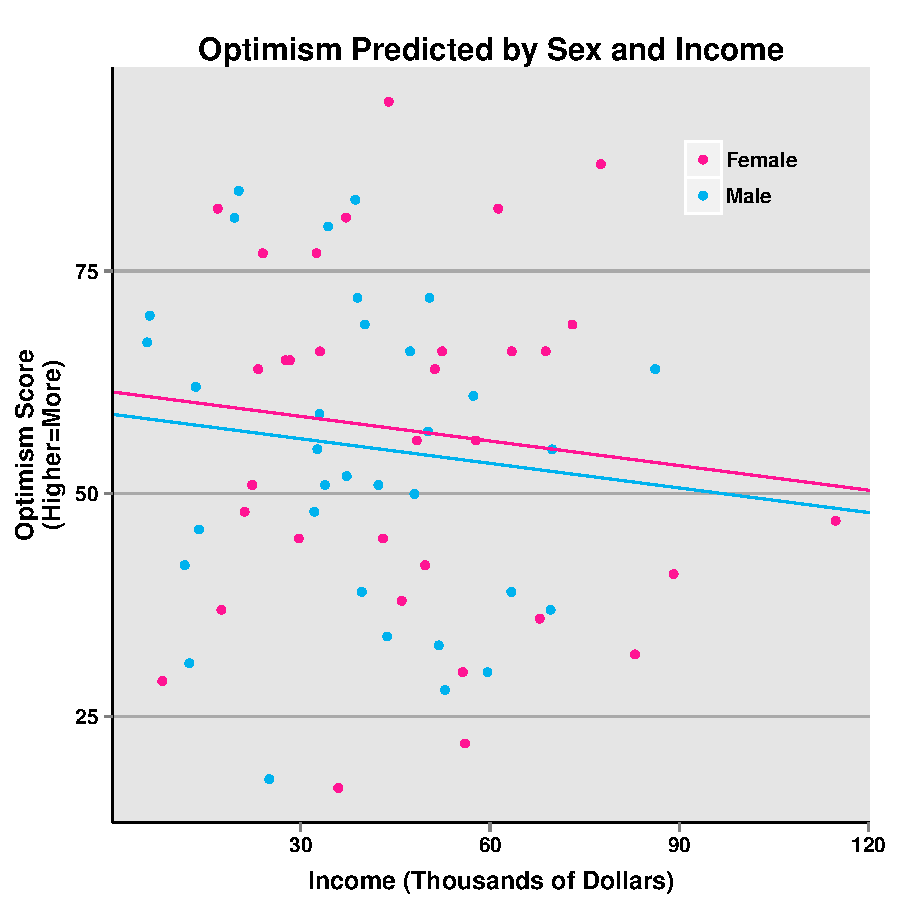
\includegraphics{Reproducibility-069}

If you included the interaction term between income and sex and found it to
be significant, you should create a linear model for each sex and create
your lines based off of those models.

\section{Summary and Homework}
Well, congratulations. You've made it through these instructions and you should
have everything you need to successfully complete the reproducibility and
statistics homework assignment. Most of you should also have everything you
need to run the analyses on the data you'll collect and create tables and / or
figures for your results.

To complete the assignment you'll need to fork my project as described above
and edit the Homework.Rmd file to run the analyses and create the figures I
request. Of course, if you have questions or problems. Contact me.

One final request. This is a work in progress. Should you find any errors,
which there inevitably will be, or any sections that could use some
improvement, \emph{please}, \href{http://wknapp.com/mailform}{let me know}!

\hfill \break
Cheers,

\hfill \break
William
\end{document}
